\documentclass[a4paper]{article}
\usepackage[utf8]{inputenc}


%=-=-=-=-=-=-=-=-=-=-=-=-=-=-=-=-=-=-=-=-=-=-=-=-=-=-=-=-=-=-=-=-=-=-=-=-=-=-=-=-
% PREAMBLE
%=-=-=-=-=-=-=-=-=-=-=-=-=-=-=-=-=-=-=-=-=-=-=-=-=-=-=-=-=-=-=-=-=-=-=-=-=-=-=-=-

%%%%%%%%%%%%%%%%%%%%%%%%%%%%%%%%%%%%%%%%%%%%%%%%%%%%%%%%%%%%%%%%%%%%%
% Important styling notes
%%
% For now, to include img.jpg in img/path/to/img.jpg, just use:
% path/to/img.jpg - for details see style.tex
%=-=-=-=-=-=-=-=-=-=-=-=-=-=-=-=-=-=-=-=-=-=-=-=-=-=-=-=-=-=-=-=-=-=-=-=-=-=-=-=-
% Packages
%%
%\usepackage{fullpage} % Package to use full page
\usepackage[top=1in,bottom=1in,left=1in,right=0.7in,heightrounded]{geometry}

\usepackage{parskip}                    % Package to tweak paragraph skipping
\usepackage{amsmath}                    % standard
\usepackage{amssymb}                    % standard - Double R symbol etc.
\usepackage{hyperref}
\usepackage{amsthm}                     % standard - theorem, definition, etc.
\usepackage{multicol}                   % multiple columns for numbering
\usepackage{enumitem}                   % standard - enumerate styles
\usepackage[utf8]{inputenc}
\usepackage{scrextend}                  % indentation
\usepackage{graphicx}                   % standard - add figures
\usepackage{float}                      % standard - figure position, use [H] option
\usepackage{pifont}                     % symbols
\usepackage{gensymb}                    % degree symbol \degree
\usepackage{xcolor}                     % bg color
\hypersetup{
    colorlinks,
    linkcolor={black!50!black},
    citecolor={blue!50!black},
    urlcolor={blue!80!black}
}
\usepackage{framed}                     % bg color
\usepackage[T1]{fontenc}                % small caps
\usepackage{sectsty}                    % headings colour
\usepackage{mathtools}                  % Loads amsmath
\usepackage{amsthm,thmtools,xcolor}     % coloured theorem
\usepackage[toc,page]{appendix}         % reference to appendix
%\usepackage{titlesec}                   % change chapter, section, etc. formats
\usepackage{xifthen}                    % if, else
\usepackage{etoolbox}
% format numbering in theorem, lemma, etc. environment
\AtBeginEnvironment{theorem}{\setlist[enumerate, 1]{font=\upshape,  wide=0.5em, before=\leavevmode}}
\AtBeginEnvironment{lemma}{\setlist[enumerate, 1]{font=\upshape,  wide=0.5em, before=\leavevmode}}
\usepackage[letterspace=150]{microtype} % \textls{<letterspaced text>} % 0 <= letterspace <= 1000, 1000 = M space
\usepackage{letltxmacro}                % renew commands?
\usepackage{minted}                     % package to list code
    % otherwise minted goes off the page
    \setmintedinline{breaklines}
\usepackage{subfig}
\usepackage{eso-pic}                    % title page bg pic
\usepackage{varwidth}
\PassOptionsToPackage{svgnames}{xcolor}
\usepackage{fontawesome}                % \faQuestionCircle
\usepackage{marvosym}                   %\Pointinghand
\usepackage{mdframed}                   % easy outline frames
\usepackage[many]{tcolorbox}            % colour box for theorem styles
\usepackage{array,booktabs,calc} % table figs and text
\usepackage{comment}                    % \begin{comment}
\usepackage{fancyhdr}                   % page headings
\usepackage{mdframed}                   % boxes
\usepackage[backend=biber,sorting=none,style=ieee]{biblatex}
\usepackage{caption}
%%% caption options {
%\DeclareCaptionFont{white}{\color{white}}
\DeclareCaptionFormat{listing}{\colorbox{magenta!30!gray}{\parbox{\textwidth}{#1#2#3}}}
\captionsetup[lstlisting]{format=listing,labelfont={bf,small},textfont=small,skip=-1pt}
%%% }
\addbibresource{bibliography.bib}
\usepackage{url}
\usepackage{textcomp}
\usepackage[makeroom]{cancel}            % crossed symbols
\usepackage{algorithm}
\usepackage[noend]{algpseudocode}
\usepackage{tikz}
\usetikzlibrary{arrows.meta,positioning,quotes} % arrows and nodes in tikz
\usepackage{marginnote}
\usepackage{pgfplots}
\usepackage{pstricks-add,pst-slpe}  % for fancy tikz arrows
%\usepackage{titlesec}                   % title style
\usepackage{lmodern}                    % a font
\usepackage{titletoc} % Required for manipulating the table of contents
\usepackage{titlesec} % Allows customization of titles
\usepackage{fouriernc} % Use the New Century Schoolbook font
\usepackage{booktabs} % things in page margins
\usepackage{stmaryrd } % \varoast
\usepackage{listings} % code listings
\usepackage{longtable} % table across multiple pages
\usepackage{styles/nasm/lang}  % include custom language for NASM assembly.
\usepackage{styles/nasm/style} % include custom style for NASM assembly.



%% extra comments that I don't know where they belong:
% list of ding tags: http://willbenton.com/wb-images/pifont.pdf

%=-=-=-=-=-=-=-=-=-=-=-=-=-=-=-=-=-=-=-=-=-=-=-=-=-=-=-=-=-=-=-=-=-=-=-=-=-=-=-=-
% Colours for various things
%%


\definecolor{shadecolor}{rgb}{1.,0.933,0.96} % bg color, r,g,b <= 1
\definecolor{medium_blue}{RGB}{60,125,190}
\definecolor{dark_blue}{RGB}{25,60,85}
\definecolor{dark_red}{RGB}{77,16,16}
\definecolor{LightPink}{rgb}{0.92.,0.8,0.84} % bg color, r,g,b <= 1
\definecolor{LighterPink}{rgb}{1.,0.94,0.97} % bg color, r,g,b <= 1
\definecolor{LightestPink}{rgb}{1.,0.95,0.99} % bg color, r,g,b <= 1
\definecolor{DarkestPink}{rgb}{0.36, 0.0, 0.18}
\definecolor{DarkerPink}{rgb}{0.41, 0.0, 0.21}
\definecolor{DarkPink}{rgb}{0.55, 0.05, 0.37}
\definecolor{lightestestpink}{RGB}{255,248,252}
\definecolor{codegray}{rgb}{0.5,0.5,0.5}
\definecolor{codegrayblue}{rgb}{0.35,0.35,0.47}



%=-=-=-=-=-=-=-=-=-=-=-=-=-=-=-=-=-=-=-=-=-=-=-=-=-=-=-=-=-=-=-=-=-=-=-=-=-=-=-=-
% Define my own theorem styles
%%

% "base" styles
\declaretheoremstyle[
  headfont=\color{DarkPink}\bfseries,
  bodyfont=\itshape,
]{colored}

\declaretheoremstyle[
  headfont=\color{DarkPink}\bfseries,
  bodyfont=\normalfont,
]{colored_upright}

% theorems (corollaries, etc) themselves, inherit from my style above
% Usage:
% \begin{theorem} \end{theorem}, \begin{lemma} \end{lemma}, ...
\declaretheorem[
	numberwithin=section,
 	style=colored,
	name=\textsc{Theorem},
]{theorem}

\tcolorboxenvironment{theorem}{
  boxrule=0pt,
  boxsep=2pt,
  colback={magenta!25!white},
  colframe=DarkPink,
  enhanced jigsaw, 
  borderline west={2pt}{0pt}{DarkPink},
  sharp corners,
  before skip=5pt,
  after skip=5pt,
  breakable,
  right=0mm % for equations
}

\declaretheorem[
	numberwithin=section,
 	style=colored,
	name=\textsc{Corollary},
]{corollary}

\tcolorboxenvironment{corollary}{
  boxrule=0pt,
  boxsep=1pt,
  colback={magenta!10!white},
  colframe=DarkPink,
  enhanced jigsaw, 
  borderline west={2pt}{0pt}{DarkPink},
  sharp corners,
  before skip=5pt,
  after skip=5pt,
  breakable,
  right=0mm % for equations
}

\declaretheorem[
	numberwithin=section,
	style=colored,
	name=\textsc{Lemma},
]{lemma}

\tcolorboxenvironment{lemma}{
  boxrule=0pt,
  boxsep=1pt,
  colback={magenta!10!white},
  colframe=DarkPink,
  enhanced jigsaw, 
  borderline west={2pt}{0pt}{DarkPink},
  sharp corners,
  before skip=5pt,
  after skip=5pt,
  breakable,
  right=0mm % for equations
}

\declaretheorem[
	numberwithin=section,
	style=colored,
	name=\textsc{Definition},
]{definition}

\tcolorboxenvironment{definition}{
  boxrule=0pt,
  boxsep=1pt,
  colback={magenta!25!white},
  colframe=DarkPink,
  enhanced jigsaw, 
  borderline west={2pt}{0pt}{DarkPink},
  sharp corners,
  before skip=5pt,
  after skip=5pt,
  breakable,
  right=0mm % for equations
}

\declaretheorem[
	numberwithin=section,
  	style=colored,
  	name=\textsc{Example},
]{exmp}

\declaretheorem[
	numberwithin=section,
  	style=colored,
  	name=\textsc{Solution},
]{soln}

%%% code listings
\lstdefinestyle{code1}{
    backgroundcolor=\color{lightestestpink},   
    commentstyle=\color{codegrayblue},
    keywordstyle=\color{DarkerPink},
    numberstyle=\tiny\color{codegray},
    stringstyle=\color{black!40!cyan},
    basicstyle=\small\ttfamily,
    breakatwhitespace=false,
    breaklines=true,        
    captionpos=t,             
    keepspaces=true,        
    numbers=left,           
    numbersep=5pt,
    showspaces=false, 
    showstringspaces=false,
    showtabs=false,
    tabsize=4
}

\lstset{style=code1}

%=-=-=-=-=-=-=-=-=-=-=-=-=-=-=-=-=-=-=-=-=-=-=-=-=-=-=-=-=-=-=-=-=-=-=-=-=-=-=-=-
% Headers (size, font, colour)
%%




\makeatletter
\renewcommand{\@seccntformat}[1]{\llap{\textcolor{DarkestPink}{\csname the#1\endcsname}\hspace{1em}}}                    
\renewcommand{\section}{\@startsection{section}{1}{\z@}
{-4ex \@plus -1ex \@minus -.4ex}
{1ex \@plus.2ex }
{\normalfont\large\sffamily\bfseries\textcolor{DarkestPink}}}
\renewcommand{\subsection}{\@startsection {subsection}{2}{\z@}
{-3ex \@plus -0.1ex \@minus -.4ex}
{0.5ex \@plus.2ex }
{\normalfont\sffamily\bfseries\textcolor{DarkestPink}}}
\renewcommand{\subsubsection}{\@startsection {subsubsection}{3}{\z@}
{-2ex \@plus -0.1ex \@minus -.2ex}
{.2ex \@plus.2ex }
{\normalfont\small\sffamily\bfseries\textcolor{DarkestPink}}}                        


%=-=-=-=-=-=-=-=-=-=-=-=-=-=-=-=-=-=-=-=-=-=-=-=-=-=-=-=-=-=-=-=-=-=-=-=-=-=-=-=-
% Numberings, counters and spacings
%%
\numberwithin{equation}{section} % section number in eq/s
\setlength{\jot}{7pt} % spacing in split, gathered env/s



%% Custom examples
%% Output - Example 1,2,...
\newcounter{example}
\newenvironment{example}[1][]{\refstepcounter{example}\par\medskip
   \textbf{Example~\theexample. #1} \rmfamily}{\medskip}
%%%%%%%%%%%% End of unused %%%%%%%%%%%%



%=-=-=-=-=-=-=-=-=-=-=-=-=-=-=-=-=-=-=-=-=-=-=-=-=-=-=-=-=-=-=-=-=-=-=-=-=-=-=-=-
% Paths
%%
\graphicspath{ {./img/} } % figures' path - can look up files directly from there


%=-=-=-=-=-=-=-=-=-=-=-=-=-=-=-=-=-=-=-=-=-=-=-=-=-=-=-=-=-=-=-=-=-=-=-=-=-=-=-=-
% User defined macros (math mode)
%%


% Curly braces under text. Usage: \myunderbrace{upper}{lower}
\newcommand{\myunderbrace}[2]{\mathrlap{\underbrace{\phantom{#1}}_{#2}} #1}
\newcommand{\setR}{\mathbb{R}} % \ouble R
\newcommand{\setRn}{\mathbb{R}^n} %  double R^n
\newcommand{\setN}{\mathbb{N}} % double N
\newcommand{\setZ}{\mathbb{Z}} % double Z
\let\oldemptyset\emptyset
\let\emptyset\varnothing % nice - looking empty set symbol
\newcommand{\fancyN}{\mathcal{N}} % null space
\newcommand{\fancyR}{\mathcal{R}} % range

\newcommand{\bx}{\textbf{x}}
\newcommand{\by}{\textbf{y}}
\newcommand{\bb}{\textbf{b}}
\newcommand{\bA}{\textbf{A}}
\newcommand{\bB}{\textbf{B}}
\newcommand{\bI}{\textbf{I}}
% double bars as in norm
\newcommand{\norm}[1] {\lVert #1 \rVert} 
\newcommand{\trans}[1]{#1^{\top}}

\newcommand{\mean}[1]{\bar{#1}}
\newcommand{\var}{\sigma^2}

\newcommand{\partdevx}[1]{\frac{\partial #1}{\partial x}}
\newcommand{\partdevxx}[1]{\frac{\partial #1}{\partial x}}
\newcommand{\partdevxn}[1]{\frac{\partial^n #1}{\partial x^n}}
\newcommand{\partdevy}[1]{\frac{\partial #1}{\partial x}}
\newcommand{\partdevyy}[1]{\frac{\partial #1}{\partial y}}
\newcommand{\partdevyn}[1]{\frac{\partial^n #1}{\partial y^n}}

% text above = symbol
\newcommand{\overeq}[1]{\ensuremath{\stackrel{#1}=}} 
\newcommand{\greatersmaller}{%
  \mathrel{\ooalign{\raisebox{.6ex}{$>$}\cr\raisebox{-.6ex}{$<$}}}
} % greater and smaller symbols on top of each other, same line

%=-=-=-=-=-=-=-=-=-=-=-=-=-=-=-=-=-=-=-=-=-=-=-=-=-=-=-=-=-=-=-=-=-=-=-=-=-=-=-=-
% User defined macros (non math)

\newcommand{\qedblack}{$\hfill\blacksquare$} % black square end of line
\newcommand{\qedwhite}{\hfill \ensuremath{\Box}} % white square end of line
\newcommand{\hquad}{\hskip0.5em\relax}% half quad space
%\newcommand{\TODO}{\textcolor{red}{\bf TODO!}\;}

\newcommand{\TODO}[1][]{%
    \ifthenelse{\equal{#1}{}}{\textcolor{red}{\bf TODO!}\;}{\textcolor{red}{\textbf {TODO:} #1}\; }%
}
\newcommand{\B}[1]{\textbf{\textup{#1}}} % bold and upright
\renewcommand{\labelitemi}{\scriptsize$\textcolor{DarkPink}{\blacksquare}$} % itemize - squares instead of bullets
\newcommand{\emphasis}[1]{\textls{#1}}

\LetLtxMacro{\originaleqref}{\eqref}
\renewcommand{\eqref}{Eq.~\originaleqref}
\renewcommand*{\eqref}[1]{Eq.~\originaleqref{#1}}





% background images
%%%%%%%
\newcommand\BackgroundPic{%
\put(0,0){%
\parbox[b][\paperheight]{\paperwidth}{%
\vfill
%\centering

\includegraphics[width=0.125\paperwidth,height=\paperheight,%
]{img/background_02.png}% use ,keepaspectratio
\vfill
}}}
%%%%%%%
% end of background image
%%%%%%%%%%%%%% my own frame
\newmdenv[topline=false,bottomline=false]{leftrightbox}
%%%%%%%%%%%%% end
%%%%%%%%%%%%% my own comment
\newcommand{\mycomment}[1]{\begin{leftrightbox}\Pointinghand~\textbf{Comment:}~#1 \end{leftrightbox}}
%%%%%%%%%%%%% end
% my custom note https://tex.stackexchange.com/questions/301993/create-custom-note-environment-with-tcolorbox
\newmdenv[
    topline=false,
    bottomline=false,
    rightline=false,
    innerrightmargin=0pt
]{siderule}
\newenvironment{mynote}%
    {\begin{siderule}\textbf{\Pointinghand~Note:}}
    {\end{siderule}}
%%%%%%%%%%%%% my own box
\newcommand{\boxone}[1]{\begin{tcolorbox}[colback = LighterPink,colframe=LightPink]
#1
\end{tcolorbox}}
%%%%%%%%%%%%% end

\let\oldemptyset\emptyset
\let\emptyset\varnothing
%algorithmic
\algdef{SE}[DOWHILE]{Do}{doWhile}{\algorithmicdo}[1]{\algorithmicwhile\ #1}%






\begin{document}
%=-=-=-=-=-=-=-=-=-=-=-=-=-=-=-=-=-=-=-=-=-=-=-=-=-=-=-=-=-=-=-=-=-=-=-=-=-=-=-=-
% GLOBAL STYLES (DOCUMENT SCOPE)
%=-=-=-=-=-=-=-=-=-=-=-=-=-=-=-=-=-=-=-=-=-=-=-=-=-=-=-=-=-=-=-=-=-=-=-=-=-=-=-=-
% caption: Figure 1 -> <bold> Fig. 1 </bold>
\captionsetup[figure]{labelfont={bf},labelformat={default},labelsep=period,name={Fig.}}


%=-=-=-=-=-=-=-=-=-=-=-=-=-=-=-=-=-=-=-=-=-=-=-=-=-=-=-=-=-=-=-=-=-=-=-=-=-=-=-=-
% TITLE PAGE
%=-=-=-=-=-=-=-=-=-=-=-=-=-=-=-=-=-=-=-=-=-=-=-=-=-=-=-=-=-=-=-=-=-=-=-=-=-=-=-=-
%%%%%%%%%%%%%%%%%%%%%%%%%%%%%%%%%%%%%%%%%
% Formal Book Title Page
% LaTeX Template
% Version 2.0 (23/7/17)
%
% This template was downloaded from:
% http://www.LaTeXTemplates.com
%
% Original author:
% Peter Wilson (herries.press@earthlink.net) with modifications by:
% Vel (vel@latextemplates.com)
%
% License:
% CC BY-NC-SA 3.0 (http://creativecommons.org/licenses/by-nc-sa/3.0/)
% 
% This template can be used in one of two ways:
%
% 1) Content can be added at the end of this file just before the \end{document}
% to use this title page as the starting point for your document.
%
% 2) Alternatively, if you already have a document which you wish to add this
% title page to, copy everything between the \begin{document} and
% \end{document} and paste it where you would like the title page in your
% document. You will then need to insert the packages and document 
% configurations into your document carefully making sure you are not loading
% the same package twice and that there are no clashes.
%
%%%%%%%%%%%%%%%%%%%%%%%%%%%%%%%%%%%%%%%%%

%----------------------------------------------------------------------------------------
%	PACKAGES AND OTHER DOCUMENT CONFIGURATIONS
%----------------------------------------------------------------------------------------



%----------------------------------------------------------------------------------------
%	TITLE PAGE
%----------------------------------------------------------------------------------------



\begin{titlepage} % Suppresses headers and footers on the title page

	\centering % Centre everything on the title page
	
	\scshape % Use small caps for all text on the title page
	
	\vspace*{\baselineskip} % White space at the top of the page
	
	%------------------------------------------------
	%	Title
	%------------------------------------------------
	
	\rule{\textwidth}{1.6pt}\vspace*{-\baselineskip}\vspace*{2pt} % Thick horizontal rule
	\rule{\textwidth}{0.4pt} % Thin horizontal rule
	
	\vspace{0.75\baselineskip} % Whitespace above the title
	
	{\LARGE COMPUTER VISION NOTES\\ \Large OBJECT LOCALISATION AND TRACKING\\} % Title
	
	\vspace{0.75\baselineskip} % Whitespace below the title
	
	\rule{\textwidth}{0.4pt}\vspace*{-\baselineskip}\vspace{3.2pt} % Thin horizontal rule
	\rule{\textwidth}{1.6pt} % Thick horizontal rule
	
	\vspace{2\baselineskip} % Whitespace after the title block
	
	%------------------------------------------------
	%	Subtitle
	%------------------------------------------------
	My personal notes on
	
	\vspace*{3\baselineskip} % Whitespace under the subtitle
	
	Object Localisation Techniques; Colour Matching, Mean Shift Tracking, Optical Flow, Lukas Kanade 
	
	\vspace*{3\baselineskip} % Whitespace under the subtitle
	
	%------------------------------------------------
	%	Editor(s)
	%------------------------------------------------
	
	By
	
	\vspace{0.5\baselineskip} % Whitespace before the editors
	
	{\normalfont \Large \mintinline{latex}{0xLeo} (\url{github.com/0xleo}) \\} % Editor list
	
	\vspace{0.5\baselineskip} % Whitespace below the editor list
	
	%\textit{The University of California \\ Berkeley} % Editor affiliation
	
	\vfill % Whitespace between editor names and publisher logo
	
	%------------------------------------------------
	%	Publisher
	%------------------------------------------------
	
	
	\vspace{0.3\baselineskip} % Whitespace under the publisher logo
	
	\today % Date
	
	{DRAFT X.YY} % Draft version
	{\\Missing: \ldots}

\end{titlepage}

%----------------------------------------------------------------------------------------

%\maketitle



%=-=-=-=-=-=-=-=-=-=-=-=-=-=-=-=-=-=-=-=-=-=-=-=-=-=-=-=-=-=-=-=-=-=-=-=-=-=-=-=-
% MAIN DOCUMENT
%=-=-=-=-=-=-=-=-=-=-=-=-=-=-=-=-=-=-=-=-=-=-=-=-=-=-=-=-=-=-=-=-=-=-=-=-=-=-=-=-
\newpage
\tableofcontents
\newpage



%------------------------------ New section ------------------------------%
\section{Principal Component Analysis}






\subsection{What is Principal Component Analysis useful for?}

Principal Component Analysis (PCA) is a statistical way to identify patterns in data. Patterns are found based on how correlated the data are. Having found such patterns, it can reduce their dimensionality.

% ref http://www.math.union.edu/~jaureguj/PCA.pdf
Suppose we have $n$ samples of $m$-dimensional data, arranged in a matrix $\bX_{n\times m}$. For example, suppose we have $n=30$ individuals and for the $i$-th individual we have recorded their height (m), weight (kg) and IQ in a vector $\bx_i \in \setR^{3}\; (m=3)$. A measurement $\bx_i$ might look like:
\[
\bx_i = \begin{bmatrix}1.8 & 70.3 & 105 \end{bmatrix}
\]
These data could be visualised as a plot of $30$ points in $\setR^3$. PCA aims to answer the following questions:
\begin{enumerate}
    \item Is there a simpler way to cluster the data? For example, if the measurements consist of 3D data, can they be clustered around a plane?
    \item Which variables are correlated? In the example, we'd expect to see correlation between weight and height but not IQ with height.
    \item Which variables are most significant when describing the dataset?
\end{enumerate}
In general, when we have $n$ measurements, each one containing $m$ variables, or ``features'' (such as height, weight, etc), we stack in what's called a data matrix.
% http://users.stat.umn.edu/~helwig/notes/datamat-Notes.pdf
\begin{definition}[data matrix]
Given $n$ measurements of $D$ variables, i.e. the measurement $i$ is $\bx_i = \begin{bmatrix}x_{i1} & x_{i2} & \ldots & x_{im}\end{bmatrix}$, the \emphasis{data matrix} contains the measurements as row vectors and the variables (features) as columns:
\begin{equation}
    \bX_{n\times m} = \begin{bmatrix}\bx_1 \\ \bx_2  \\ \vdots \\ \bx_n \end{bmatrix} = 
    \begin{bmatrix}
    x_{11} & x_{12} & \ldots & x_{1D} \\
    x_{21} & x_{22} & \ldots & x_{2D} \\
    \vdots & \vdots & \ddots & \vdots \\
    x_{n1} & x_{n2} & \ldots & x_{nD}
    \vdots
    \end{bmatrix}
\end{equation}
\end{definition}
For instance, for our (height, weight, IQ) data, a toy data matrix would contain the measurements as rows and the \textit{variables} (``features'') as \textit{columns}:
\[
\bX = \begin{bmatrix}
1.88 & 96 & 91 \\
1.90 & 78 & 125 \\
1.72 & 84 & 114 \\
1.79 & 89 & 100 \\
1.77 & 77 & 93 \\
\end{bmatrix}
\begin{array}{l}
    \leftarrow \textup{measurement\; 1}  \\
    \leftarrow \ldots  \\
    \leftarrow \ldots  \\
    \leftarrow \ldots  \\
    \leftarrow \textup{measurement\; 5}  \\
\end{array}
\]





\subsection{Required background}

Before we study PCA, we need some linear algebra and statistics background. Proofs are left to the reader. Some data science and statistics terminology is also used.

% ref http://www.math.union.edu/~jaureguj/PCA.pdf
\begin{lemma} If $\bA \in \setR^{n\times D}$, then matrices $AA^{T} \in \setR^{n\times n}$ and  $A^{T}A \in \setR^{D\times D}$. Furthermore, $AA^{T}$ and $A^{T}A$ share the same, non-zero, eigenvalues. 
\end{lemma}
\marginnote{Don't get confused with the notation; $\left[
x_{i1} \; \ldots \; x_{in}
\right]\t$ $=\begin{bmatrix}
x_{1i} \\ \vdots \\ x_{ni}
\end{bmatrix}$ refers to the $i$-th column (feature) of the data matrix.}
\begin{lemma}
The eigenvalues of $A\t A$ and $AA\t$ are non-negative.
\end{lemma}
In PCA, which is studied later, we often have a ``fat'' matrix $\bA$ of size $M\times N, \quad N \gg M$ and want to find the eigenvalues of the product $\bA\t\bA$. Note that $\bA\t\bA$ is of size $N\times N$, so e.g. for $N=1000$, it is impractical to directly perform eigen-analysis on  $\bA\t\bA$ -- a $1000\times 1000$ matrix! Instead, we perform it on $\bA\bA\t\in \setR^{M\times M}$ and leverage a relationship between the eigendata of $\bA\t\bA$ and $\bA\bA\t$.
\begin{lemma}[Eigenvalues of $\bA\t\bA$ and $\bA\bA\t$]
\label{lem:eig_ata_aat}
	Let $\bA \in \setR^{M\times N}$ and $\lambda_i, \; \bu_i$	be the eigenvalues and eigenvectors of $\bA\t\bA$. If $\mu_i$ and $\textbf{v}_i$ are the eigenvalues and eigenvectors of $\bA\bA\t$, then the eigendata of $\bA\t\bA$ are given by:
	\begin{align}
		\lambda_i = \mu_i & & & \bu_i = \bA\t\textbf{v}_i
	\end{align}
\end{lemma}
\begin{proof}
	Since $\textbf{v}_i$ and $\mu_i$ are the eigendata of $\bA\bA\t$:
	\begin{align*}
		\bA\bA\t\textbf{v}_i = \mu_i\textbf{v}_i \Rightarrow \\
		\bA\t\bA\underbrace{\bA\t\textbf{v}_i}_{\bu_i} = \underbrace{\mu_i}_{\lambda_i}\underbrace{\bA\t\textbf{v}_i}_{\bu_i}
	\end{align*}
	The last relationship precisely tells us that the eigenvalues of $\bA\t\bA$ are $\lambda_i=\mu_i$ and the its eigenvectors are $\bu_i = \bA\t\textbf{v}_i$.
\end{proof}


The following definitions from statistics will be required.
\begin{definition}[mean of feature] Let $\bX \in \setR^{n \times D}$ be the data matrix. Each column contains a feature $\bx_i$ of $n$ entries with $\bx_{i}  = \begin{bmatrix}x_{i1} & x_{i2} & \ldots & x_{in}\end{bmatrix}\t$. Then we define the \emphasis{mean} of feature $j$ as its average: 
\begin{equation}
    \bar{x}_j = \frac{1}{n}\sum\limits_{i=1}^{n}x_{ij}
    \label{eq:def_mean_vector}
\end{equation}
\end{definition}
\begin{definition}[variance]
Given a feature $\bx_j \in \setR^{n\times 1}$ in the data matrix with entries $x_{1j},\ldots,x_{nj}$ and mean $\bar{x}_j$, its \emphasis{sample variance} $\sigma_{\bx_i}^2$ is defined as:
\begin{equation}
   \sigma_{\bx_j}^2 = \frac{1}{n-1}\sum\limits_{i=1}^{n} (x_{ij} - \bar{x_j})^2
\end{equation}
\end{definition}
Variance of a feature measures its spread.Variance of a feature measures its spread.


\begin{definition}[covariance]
Given two features (column vectors in data matrix) $\bx_j,\bx_k$ with entries $\begin{bmatrix}x_{j1} & x_{j2} & \ldots & x_{jn}  \end{bmatrix}\t$, $\begin{bmatrix}x_{k1} & x_{k2} & \ldots & x_{kn}  \end{bmatrix}\t$ respectively and means $\bar{x_j},\ \bar{x_k}$ respectively, their \emphasis{covariance} is defined as:
\begin{equation}
    \sigma(x_j,x_k) = \frac{1}{n-1}\sum\limits_{i=1}^{n}(x_{ij} - \bar{x_j})(x_{ik} - \bar{x_k})
\end{equation}
\end{definition}
Notice how the covariance of $x_j$ with itself is its variance. Covariance provides intuition regarding the dispersion of $\bx_j$ and $\bx_k$ -- i.e. how they change with respect to one another;
\begin{itemize}
    \item Covariance $\sigma(\bx_j,\bx_k)$ is positive when variables $\bx_j,\bx_k$ ``move together''.
    \item Covariance is negative when $\bx_j,\bx_k$ ``move inversely''.
    \item Covariance is zero when $\bx_j,\bx_k$ move randomly w.r.t. each other, i.e. they are ``uncorrelated'' (fancy word for unrelated).
\end{itemize}
\begin{figure}[H]
    \centering
    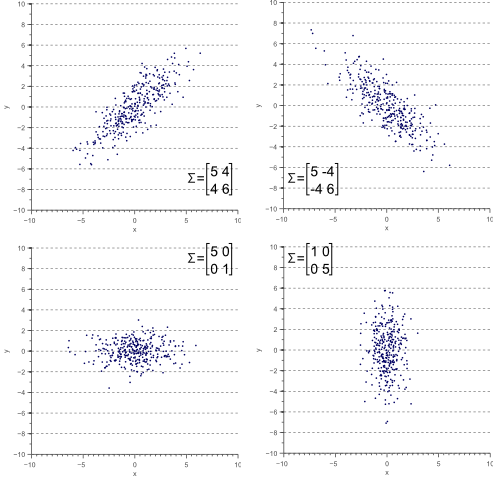
\includegraphics[height=7cm]{img/covariance_matrices_2d_points.png}
    \caption{Some covariance matrices $\Sigma$ for various 2D datasets. Observe how the matrix values are related to the shape  (\url{https://pathmind.com/wiki/eigenvector}).}
    \label{fig:my_label}
\end{figure}
From the definition, it is straightforward that the covariance function is symmetric.
\begin{corollary}[covariance is symmetric]
For the covariance of any two feature vectors $\bx_k$, $\bx_k\in \setR^{n\times 1}$:
\begin{equation}
    \sigma(\bx_j,\bx_k) = \sigma(\bx_j,\bx_k)  
\end{equation}
\end{corollary}
If we have multi-dimensional data, let's say $n$ measurements of $m$-dimensional data, we compute the ``covariance matrix'' as follows.
\begin{definition}[covariance matrix]
% ref http://users.stat.umn.edu/~helwig/notes/datamat-Notes.pdf
\marginnote{Each entry $jk$ of the covariance matrix contains the covariance between two feature vectors $\bx_j,\ \bx_k$, $1\leq j,k \leq m$}Given $n$ observations of $D$-dimensional variables, their \emphasis{covariance matrix} $\bSigma\in \setR^{D\times D}$ refers to the symmetric array of numbers:
\begin{equation}
    \bSigma = 
    \frac{1}{n-1}
    \begin{bmatrix}
    \sigma_1^2 & \sigma_{12} & \ldots & \sigma_{1D}\\
    \sigma_{21} & \sigma_2^2 & \ldots & \sigma_{2D}\\
    \vdots & \vdots & \ddots & \vdots \\
    \sigma_{D1} & \sigma_{D2} & \ldots & \sigma_D^2 
    \end{bmatrix}
    \label{eq:cov_alg_form}
\end{equation}
, where
% ref http://users.stat.umn.edu/~helwig/notes/datamat-Notes.pdf
\begin{itemize}
    \item $\sigma_j^2 = \frac{1}{n-1}\sum\limits_{i=1}^{n}(x_{ij} - \bar{x}_j)^2$ is the variance of the $j$-th variable.
    \item $\sigma_{jk}^2 = \frac{1}{n-1}\sum\limits_{i=1}^{n}( x_{ik} - \bar{x}_j)(x_{ik} - \bar{x}_k)$ is the covariance between variables $j$ and $k$.
\end{itemize}
\end{definition}

We will now show how the covariance matrix $\boldsymbol{\sigma}$ can be computed from the data matrix $\bX$ using matrix operations. We defined in \eqref{eq:def_mean_vector} the mean vector of all features as:
\[
\bar{\bx} = \begin{bmatrix}\bar{x}_1 \\ \vdots \\ \bar{x}_D \end{bmatrix}, \quad
\bar{x}_j  = \frac{1}{n}\sum\limits_{i=1}^{n}x_{ij} 
\]
It can be easily verified that $\bar{\bx}$ can be computed in terms of $\bX$ as:
\begin{gather*}
    \bar{\bx} = n^{-1}\bX\t\textbf{1}_{n\times 1} \tag{\ding{168}}
    \label{eq:cov_proof_x_bar_wrt_x}
\end{gather*}
% https://shreydesai.github.io/2019/02/14/principal_component_analysis.html
, where $\textbf{1}_{n\times 1}$ is a column vector of ones. The covariance matrix can also be written in terms of the ``centred'' (zero mean) matrix $\bX_C$
\[
\boldsymbol{\sigma}(\bX) = n^{-1}\bX_c\t\bX_c, \quad \bX_c = 
\begin{bmatrix}
x_{11} - \bar{x_1} & x_{12} - \bar{x_2} & \ldots & x_{1p} - \bar{x_p}\\
x_{21} - \bar{x_1} & x_{22} - \bar{x_2} & \ldots & x_{2p} - \bar{x_p}\\
\vdots & \vdots & \ddots & \vdots \\
x_{n1} - \bar{x_1} & x_{n2} - \bar{x_2} & \ldots & x_{np} - \bar{x_p}\\
\end{bmatrix} = 
\bX - 
\begin{bmatrix}
\bar{x_1} & \bar{x_2} & \ldots & \bar{x_p} \\
\vdots & \vdots & \ddots & \vdots \\
\bar{x_1} & \bar{x_2} & \ldots & \bar{x_p} \\
\end{bmatrix} 
= \bX - \textbf{1}_{n}\bar{\bx}\t
\]
\begin{gather*}
    \therefore \bX_C = \bX - \textbf{1}_{n\times 1}\bar{\bx}\t \tag{\ding{168}\ding{168}}
    \label{eq:cov_proof_cov_x_bar}
\end{gather*}
, where $\bar{\bx} = \begin{bmatrix}\bar{x}_1 & \ldots & \bar{x}_p \end{bmatrix}\t$ is the vector of the feature means and $ \textbf{1}_{n}$ is a $n\times 1$ vector of ones. For instance, if the means vector was $\bar{\bx} = \begin{bmatrix}1 & 2 & 3 \end{bmatrix}\t$, then the result $\textbf{1}_{4\times 1} \bar{\bx}\t$ would be:
\[
\begin{bmatrix}
1 \\
1 \\
1 \\
1 \\
\end{bmatrix}_{4\times 1}
\begin{bmatrix}
1 & 2 & 3
\end{bmatrix}_{1\times 3} = 
\begin{bmatrix}
1 & 2 & 3\\
1 & 2 & 3\\
1 & 2 & 3\\
1 & 2 & 3\\
\end{bmatrix}_{4\times 3}
\]
Remember, the goal is to express $\boldsymbol{\bSigma}$ in terms of $\bX$. What's left is to express $\bar{\bx}$ in terms of $\bX$. Substituting \eqref{eq:cov_proof_x_bar_wrt_x} in \eqref{eq:cov_proof_cov_x_bar}:
\begin{align*}
\bX_C &= \bX - n^{-1} \textbf{1}_{n\times 1} \textbf{1}_{n\times 1}\t \bX = \\
&= (\textbf{I}_n - n^{-1} \textbf{1}_{n\times 1} \textbf{1}_{n\times 1}\t) \bX
= C\bX, \quad \bC:= \textbf{I}_n - n^{-1} \textbf{1}_{n\times 1} \textbf{1}_{n\times 1}\t
\end{align*}
To recap, we found how the ``centred'' version of the data matrix $\bX\in \setR^{n\times D}$ can be obtained as a product. The centred $n\times D$matrix $\bX_C$ contains the centred features (columns). Centring implies that the mean of each feature is zero and as we'll see later this simplifies the PCA calculations.
\begin{equation}
    \bX_C = C\bX, \quad \bC:= \textbf{I}_n - n^{-1} \textbf{1}_{n\times 1}
    \label{eq:centred_matrix_wrt_original}
\end{equation}
Since $\bSigma$ is expressed w.r.t $\bX_C$, it's straightforwardd to express it w.r.t the original data matrix $\bX$.
\[
\therefore \bSigma(\bX) = \bX_C\t\bX_C = (n-1)^{-1}(\textbf{C}\bX)\t\textbf{C}\bX = (n-1)^{-1}\bX\t\textbf{C}\t\textbf{C}\bX
\]
To reiterate, we established that the covariance matrix can be efficiently computed as a product containing the data matrix and a constant one. 
\begin{corollary}[covariance matrix as product]
% ref http://users.stat.umn.edu/~helwig/notes/datamat-Notes.pdf
If the data matrix is $\bX_{n\times p}$, whose its columns contain features, the covariance matrix can be computed as the product:
\begin{equation}
    \bSigma = (n-1)^{-1}\bX\t\textbf{C}\t\textbf{C}\bX, \quad \textbf{C} = \textbf{I}_n - n^{-1} \textbf{1}_{n\times 1} \textbf{1}_{n\times 1}\t
    \label{eq:eq_cov_mat_def}
\end{equation}
\end{corollary}
We can quickly verify the validity of this by comparing with Matlab/ Octave's \texttt{cov} command.
\begin{verbatim}
>> X = [189 77 119;170 74 122;185 72 91;172 94 115]; % data matrix
>> n = size(X, 1);
>> C = eye(n) - 1/n*ones(n,1)*ones(n,1)';
>> cov_mat_form = 1/(n-1)*X'*C'*C*X;   
>> cov_mat_form./cov(X) % divide element-wise
ans =
   1.00000   1.00000   1.00000
   1.00000   1.00000   1.00000
   1.00000   1.00000   1.00000
\end{verbatim}



\subsection{The idea behind PCA}

PCA aims to reduce the dimensionality of the input data by projecting the $D$-dimensional input data to a $d$-dimensional space, $d\leq D$. First, the data are projected on a $D$-dimensional  space spanned by some vectors $\bu_1,\ldots,\bu_D$. Basis vectors $\bu_1,\ldots,\bu_D$ fit along the most important directions of the projected data by mapping (projecting) the original data onto the vectors. Fitting a vector along the most important direction of the original data is expressed as maximising the variance of the points $\bx_i \in \setR^D$ projected along it. Having fit the data by projecting it, the next step PCA does it to keep only the $d$ first most important projected vectors, projected along $\bu_1,\ldots,\bu_d$.

Fig. \ref{fig:pca_2d_to_1d} shows how such a vector (PC1) would look like if we wanted to fit it so that the variance of the points projected to it is maximised. If we only use PC1 to represent the compressed data, we have reduced it from a 2D representation to 1D ($D=2, d=1$). So instead of reporting its 2D position, we can report its position (scalar) on the line, assuming the PC1 line is the new axis. 
\begin{figure}[H]
    \centering
    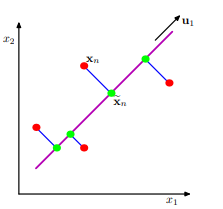
\includegraphics[height=4.25cm]{img/project_data_to_1d.PNG}
    \caption{Orthogonally projecting 2D data along an 1D line spanned by $\bu_1$.}
    \label{fig:pca_2d_to_1d}
\end{figure}


\subsection{Problem formulation and objective}
Before performing PCA, we always centre the data so that the basis they are represented by starts from the origin. Suppose our data consists of $n$ $D$-dimensional observations $\bx_1,\ldots,\bx_n$, $\bx_i\in\setR^D$. We want to project them in an orthonormal basis $\bu_1,\ldots,\bu_D$ such that the projected points have certain properties.
% ref https://alliance.seas.upenn.edu/~cis520/wiki/index.php?n=Lectures.PCA
\begin{definition}[PC loadings]
The orthonormal basis vectors $\bu_1,\ldots,\bu_D$ that form the basis of the projected data $\bx_1,\ldots,\bx_n, \; \bx_i\in\setR^D$ are called \emphasis{PC loadings}.
% ref https://www.cs.cmu.edu/~mgormley/courses/10701-f16/slides/lecture14-pca.pdf
\begin{equation}
    \bu_i\t\bu_j= \left\{
\begin{array}{ll}
      1 & i=j \\
      0 & i\neq j \\
\end{array} 
\right.
\end{equation}
\end{definition}
Projected and spanned by the basis $\bu_1,\ldots,\bu_D$, a data point $\bx\in \setR^D$ is written as:
\begin{equation*}
    \bx = \sum\limits_{i=1}^{D}(\bx\t\bu_i)\bu_i
\end{equation*}
% ref https://www.doc.ic.ac.uk/~dfg/ProbabilisticInference/IDAPISlides14.pdf
, where $(\bx\t\bu_i)\bu_i$ is its projection along axis $\bu_i$.
The objective of PC is to approximate each data vector $\bx$ at a lower-dimensional subspace using as few subspace basis vectors as possible, i.e.
\begin{equation}
    \hat{\bx} = \sum\limits_{i=1}^{d}(\bx\t\bu_i)\bu_i , \quad d \leq D
\end{equation} 


% ref https://www.cs.colostate.edu/~cs545/fall16/lib/exe/fetch.php?media=wiki:14_pca.pdf
\begin{corollary}[objective of PCA -- minimise the reconstruction error]
The orthogonal \emphasis{reconstruction error} for one centred data vector $\bx$ is defined as:
\begin{equation}
    E(\bx) = \norm{\hat{\bx}- \bx}^2 = \sum\limits_{i=d+1}^D  (\bx\t\bu_i)^2
\end{equation}
The total reconstruction error $\mathcal{L}(\bu_1,\ldots,\bu_d)=\sum\limits_{i=1}^n E(\bx_i;\bu_1,\ldots,\bu_d) = \sum\limits_{j=1}^n\sum\limits_{i=d+1}^D(\bx_j\t\bu_i)^2$ is what we strive to minimise.
\end{corollary}
 We minimise it by choosing appropriate basis vectors $\bu_1,\ldots,\bu_d$. In the next section, we will see how these vectors  should be chosen if we have a pre-defined value of $d$. Later we will also see how many PC loadings should be chosen to have a ``good enough'' representation of the original data, i.e. what the value of $d$ should be.
 
 As mentioned, PCA orthogonally projects the data from a space of dimensionality $D$ to one of $d,\; d \leq D$. Projection is accomplished as a linear operation.
 % http://lasa.epfl.ch/teaching/lectures/ML_Msc/Slides/PCA.pdf
 Remember, if $\bX = \begin{bmatrix}\bx_1 & \dots & \bx_n \end{bmatrix}$ be a matrix that contains $D$-dimensional measurements $\bx\in\setR^D$, $i=1,\ldots,n$. A projection $\textbf{Y}$ of $\bX$ through a linear map $\textbf{A}:\setR^D\rightarrow \setR^d$ is given by:
 \begin{align}
     \underset{(d\times n)}{\textbf{Y}} &= 
     \underset{(d\times D)}{\textbf{A}}
     \cdot
     \underset{(D\times n)}{\textbf{X}}
\end{align}
 
 \begin{exmp}

 For example, suppose we shave some 3D observations centred around 8 clusters:
 \[
 \bX =
 \begin{bmatrix}
 0 & 0 & 0 & 0 & 15 & 15 & 15 & 15 & 0 & 15\\
 0 & 0 & 15 & 15 & 0 & 0 & 15 & 15 & 15 & 0\\
 0 & 15 & 0 & 15 & 0 & 15 & 0 & 15 & 15 & 15\\
 \end{bmatrix}
 \]
 Let's the try multiplying by an arbitrary projection matrix $\bA$, then the output is:
 \[
 \bA = \begin{bmatrix}
 0 & 1 &0 \\1 &0 &0
 \end{bmatrix}, \quad \bY = \textbf{AX} =
 \begin{bmatrix}
 0 &0 &15 &15 &0 &0 &15 &15 &15 &0\\
 0 &0 &0 &0 &15 &15 &15 &15 &0 &15
 \end{bmatrix}
 \]
 Visually, the projection matrix reduces the data from a cube to a square:
 \begin{multicols}{2}
\begin{figure}[H]
    \centering
    %%%
% credits: https://tex.stackexchange.com/questions/431093/3d-cartesian-coordinate-system


\scalebox{0.35}{ %%% scalebox
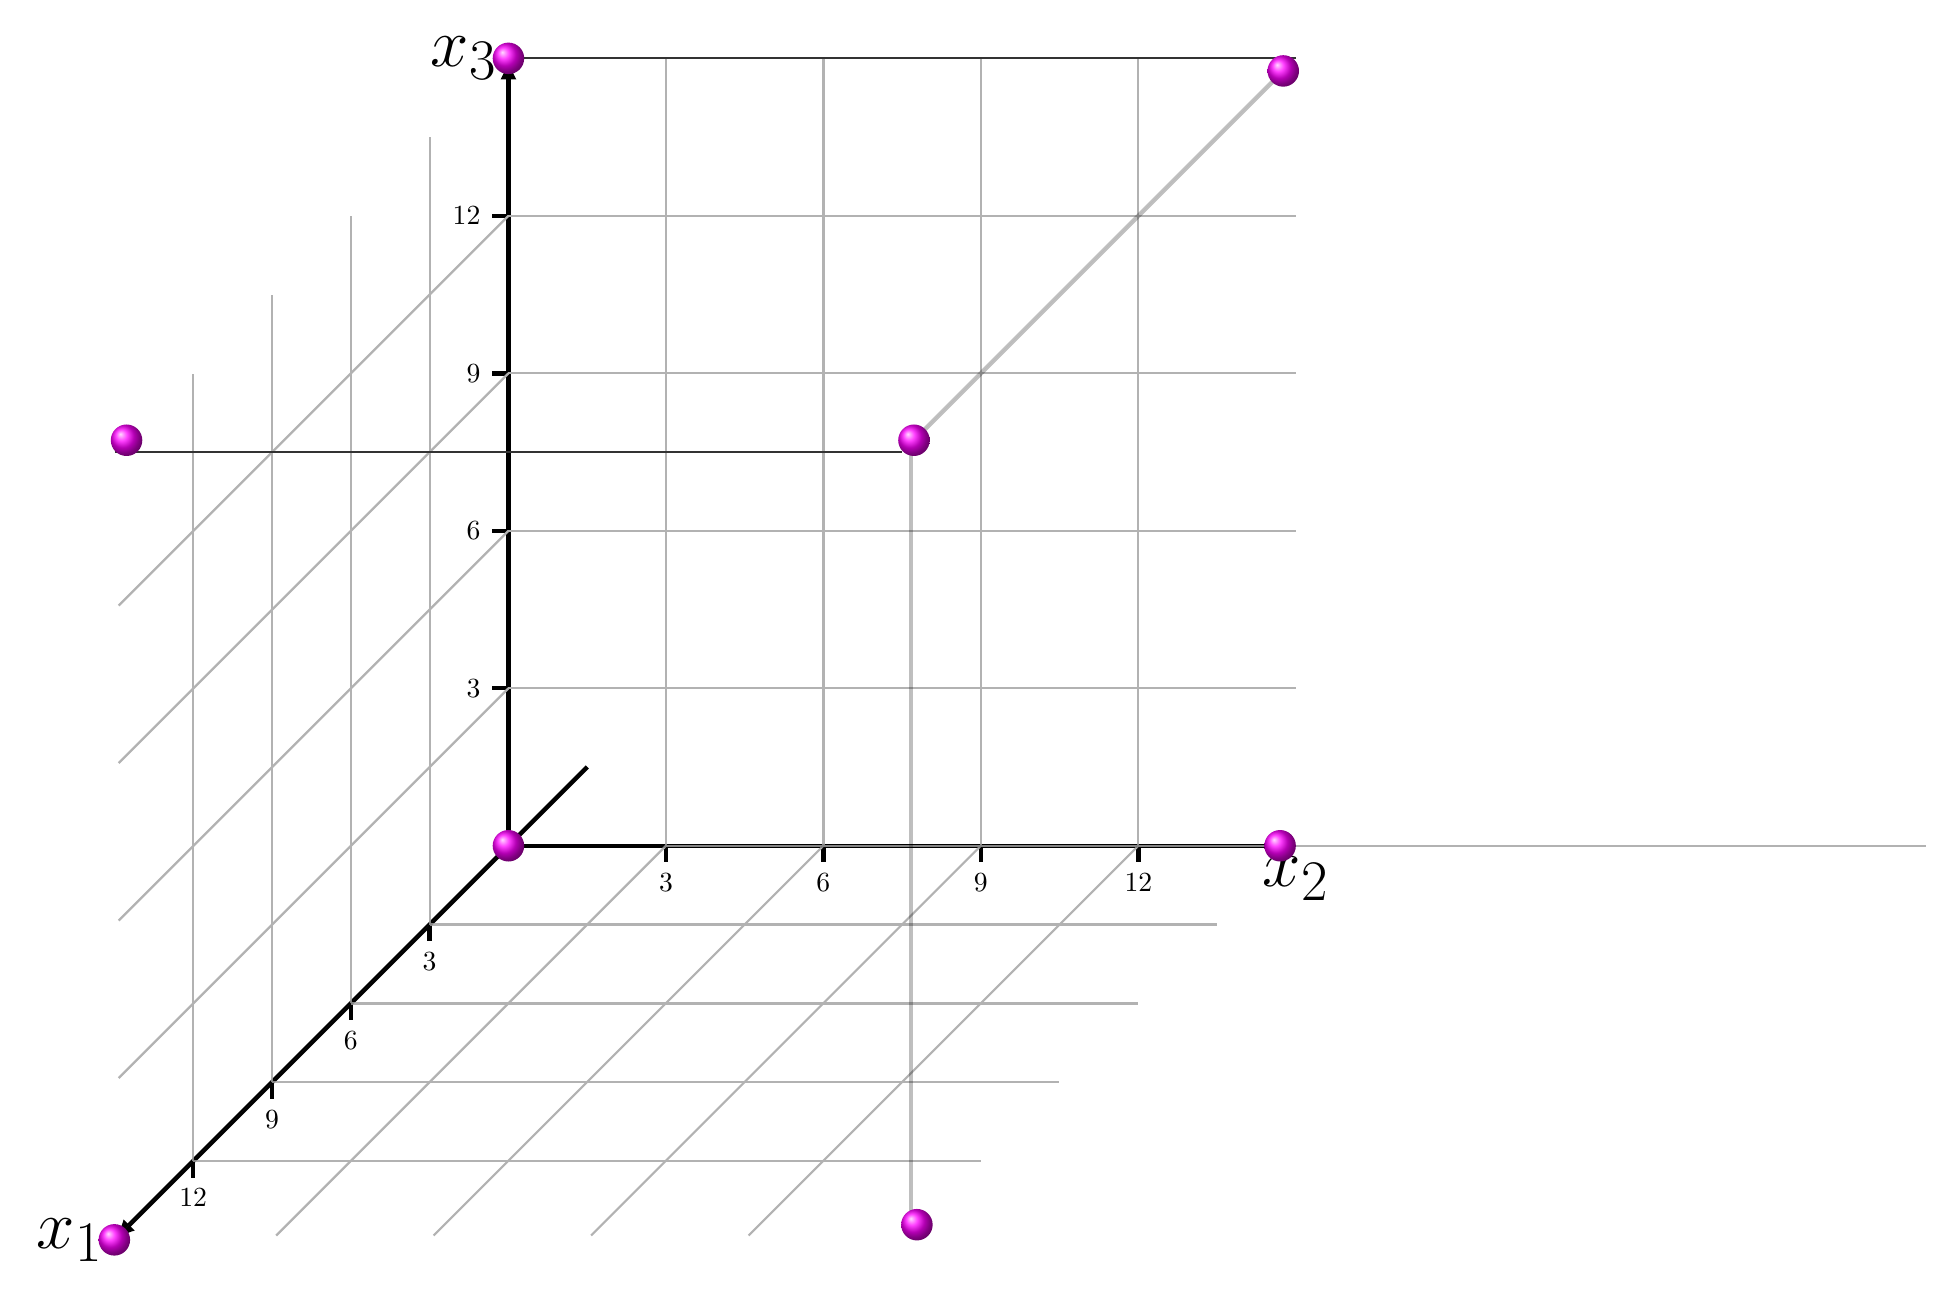
\begin{tikzpicture}
    %\draw[gray!60!white, thick] (-4.99,-4.99) grid (9.99,9.99);
    \draw[->, >=latex, ultra thick] (0,0,-2.6) -- (0,0,13) node[left]{\Huge{$x_1$}};
    \draw[->, >=latex, ultra thick] (0,0,0) -- (10,0,0) node[below]{\Huge{$x_2$}};
    \draw[->, >=latex, ultra thick] (0,0,0) -- (0,10,0) node[left]{\Huge{$x_3$}};
    % grid lines and axis ticks
    \foreach \z/\zc in {2.6/3,5.2/6,7.8/9,10.4/12}{
        \draw[shift={(0,0,\z)}, ultra thick] (0pt,0pt,0pt) -- (0pt,-0.21pt,0pt)node[below]{\zc};
        \draw[gray!60!white, thick](0,0,\z)--++(0:10);
        \draw[gray!60!white, thick](0,0,\z)--++(90:10);
    }
    \foreach \x/\xc in {2/3,4/6,6/9,8/12}{
        \draw[shift={(\x,0)}, ultra thick] (0pt,0pt) -- (0pt,-6pt)node[below]{\xc};
        \draw[gray!60!white, thick](\x,0)--++(0:10);
        \draw[gray!60!white, thick](\x,0)--++(90:10);
        \draw[gray!60!white, thick](\x,0)--++(-135:7);
    }
    \foreach \y/\yc in {2/3,4/6,6/9,8/12}{
        \draw[shift={(0,\y)}, ultra thick] (0pt,0pt) -- (-6pt,0pt)node[left]{\yc};
        \draw[gray!60!white, thick](0,\y)--++(0:10);
        \draw[gray!60!white, thick](0,\y)--++(-135:7);
    }
    %aux grid lines
    \draw[black!80!white, thick](0,10)--++(0:10);
    \draw[black!80!white, thick](-5,5)--++(0:10);
    
    % 3 planes
    \draw[fill=black!30, ultra thick, nearly transparent] (0,0,0) -- (0,0,12.7);
    \draw[fill=black!30, ultra thick, nearly transparent] (0,0,0) -- (9.9,0,0);
    \draw[fill=black!30, ultra thick, nearly transparent] (9.9,9.9,0) -- (9.9,9.9,12);
    \draw[fill=black!30, ultra thick, nearly transparent] (10,0,12.7) -- (10,10,12.7);
    % points
    \shade[ball color=magenta] (16,16,16) circle (0.2);
    \shade[ball color=magenta] (9.8,0,0) circle (0.2);
    \shade[ball color=magenta] (0,0,13) circle (0.2);
    \shade[ball color=magenta] (9,9,10) circle (0.2);
    \shade[ball color=magenta] (0,10,0) circle (0.2);
    \shade[ball color=magenta] (-1,9,10) circle (0.2);
    \shade[ball color=magenta] (10,0,12.5) circle (0.2);
    \shade[ball color=magenta] (0,0,0) circle (0.2);
\end{tikzpicture}
} % scale

    \caption{Original data; 10 observations of 3D data as 8 clusters.}
\end{figure}
\columnbreak
\begin{figure}[H]
    \centering
    

\scalebox{0.65}{ %%% scalebox
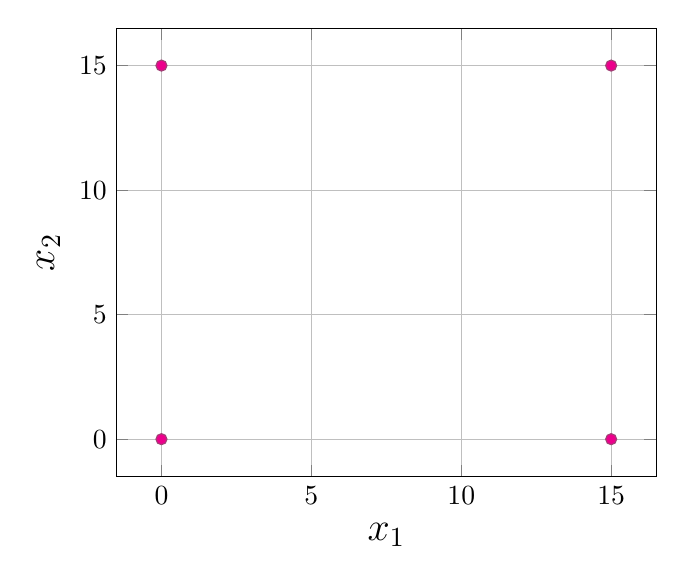
\begin{tikzpicture}
  \begin{axis}[
    xlabel=\Large{$x_1$},
    ylabel=\Large{$x_2$},
    grid=major]
    \addplot [only marks, draw=magenta!60!black, fill = magenta] coordinates {(0,0) (15,15) (15,0) (0,15)};
    % if you want the plot to be RED, instead write: \addplot [red,mark=*] coordinates ...
  \end{axis}
\end{tikzpicture}
}
    \caption{The same data after being multiplied by the $2\times 3$ projection matrix $\bA$.}
\end{figure}
\end{multicols}
 \end{exmp}
 
 \begin{mynote}
In the next sections, we will assume that $d=D$ unless otherwise specified. We will study how to compress from $D$ principal components to $d$ later.
\end{mynote}
 
 
 
 
 
\subsection{Minimising error $\Leftrightarrow$ project variance maximisation -- intuition for one PC}

%\url{http://lasa.epfl.ch/teaching/lectures/ML_Msc/Slides/PCA.pdf} very clear\\
%\url{http://ce.sharif.edu/courses/94-95/1/ce717-2/resources/root/Lectures/PCA%20&%20ICA.pdf}\\
%\url{http://www.stat.cmu.edu/~cshalizi/uADA/12/lectures/ch18.pdf}\\
%\url{http://jupiter.math.nctu.edu.tw/~yuhjye/assets/file/teaching/2017_machine_learning/PCAsubset.pdf}\\
%\url{https://www.cs.cmu.edu/~mgormley/courses/10701-f16/slides/lecture14-pca.pdf}\\
%\url{http://lcsl.mit.edu/courses/mlcc/mlcc2017/slides/MLCC_PCA.pdf}\\
%\url{https://cse.iitk.ac.in/users/piyush/courses/ml_autumn16/771A_lec11_slides.pdf}\\
%\url{https://www.cs.princeton.edu/courses/archive/fall18/cos324/files/pca.pdf}\\

\marginnote{To simplify the derivations in this section, we assume zero-mean ($\bar{\bx_i}=0$) data.}
In this section, we see what statistical properties the PCs must satisfy in order to minimise the reconstruction error. To simplify the derivations, we assume we want to project to 1D data, spanned by a single PC $\bu$. Lemmas will be generalised in another section. We assume the original data points are $D$-dimensional but they will be visualised as 2D for simplicity. Finally, we assume that the data have been centred.



\begin{figure}[H]
    \centering
    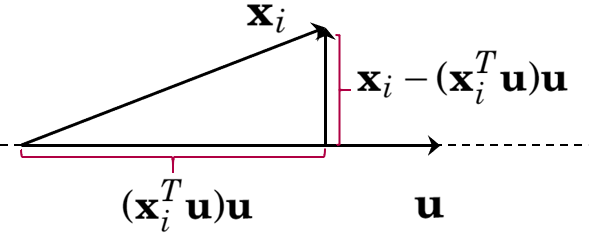
\includegraphics[height=2.3cm]{img/recon_error_for_vector.png}
    \captionsetup{width=.55\linewidth}
    \caption{Given a data vector $\bx_i$ and a (unit vector) PC loading $\bu$, the reconstruction error for $\bx_i$ is $\norm{\bxi - (\bxi\t\bu)\bu}^2$.}
\end{figure}

For data projected along a single line spanned by $\bu$, maximising the variance of the projected data minimises the reconstruction error.

% ref http://lcsl.mit.edu/courses/mlcc/mlcc2017/slides/MLCC_PCA.pdf
\begin{lemma}[variance maximisation  $\Leftrightarrow$ reconstruction error minimisation for one PC] Maximising the variance $\frac{1}{n}\sum\limits_{i=1}^{n}(\textbf{u}^T\bx_i)^2$ for the projected data,  is equivalent to minimising the total \emphasis{ reconstruction error} (a.k.a. Mean Squared Error), which is defined in as:
\begin{equation*}
    MSE = \frac{1}{n}\sum\limits_{i=1}^{n}\norm{\bx_i - (\bx_i\t\textbf{u}_1)\textbf{u}_1}^2
\end{equation*}
\end{lemma}
% ref http://www.stat.cmu.edu/~cshalizi/uADA/12/lectures/ch18.pdf
\begin{proof}
For one data vector $\bx_i$, the squared reconstruction error is:
\begin{align*}
   \norm{\bx_i - (\bx_i\t\textbf{u})\textbf{u}}^2 
   &= \left(\bx_i - (\bx_i\t\textbf{u})\textbf{u}\right)\t \left(\bx_i - (\bx_i\t\textbf{u})\textbf{u}\right) \\
   &= \bxi\t\bxi - \bxi\t\bu(\bxi\t\bu) - (\bxi\t\bu)\bu\t\bxi + (\bxi\t\bu)\bu\t\bu(\bxi\t\bu) \\
   &= \norm{\bxi}^2 - 2(\bxi\t\bu)^2 + (\bxi\t\bu)^2 \\
   &= \norm{\bxi}^2 - (\bxi\t\bu)^2
\end{align*}
, as $(\bxi\t\bu1)$ is a scalar, $\bxi\t\bu = \bu\t \bxi$, and $\bu\t\bu = \norm{\bu}_1^2 = 1$. To obtain the MSE  we sum over the $n$ data points:
\[
    MSE = \frac{1}{n} \sum\limits_{i=1}^n\norm{\bx_i - (\bx_i\t\textbf{u})\textbf{u}}^2  = \frac{1}{n}\left(\sum\limits_{i=1}^n\norm{\bxi}^2 - \sum\limits_{i=1}^n (\bxi\t\bu)^2\right)
\]
The former term is constant and the latter (assuming centred data) is $\sigma_{\bu}^2$. The proof is done.
\end{proof}



% ref http://www.bbk.ac.uk/ems/faculty/brooms/teaching/SMDA/SMDA-02.pdf





\subsection{Mathematical properties of PC's}

% visual:
% https://health.uconn.edu/bioinformatics/wp-content/uploads/sites/162/2017/11/PCA_2016.pdf
% http://users.stat.umn.edu/~helwig/notes/pca-Notes.pdf
% https://www.cs.ox.ac.uk/people/james.worrell/SVD-thin.pdf
% http://www.bbk.ac.uk/ems/faculty/brooms/teaching/SMDA/SMDA-02.pdf
% https://www.ibmm.unibe.ch/unibe/portal/fak_naturwis/a_dept_math/a_dept_ms/content/e237483/e237655/e243381/e281679/files281689/Chap8-10_ger.pdf
% https://shreydesai.github.io/2019/02/14/principal_component_analysis.html

Before we derive the other PCs, we describe the properties they must satisfy.
\marginnote{For these expressions to be true, features must be centred and in columns.}Again, let $\bX = \begin{bmatrix} \bx_1,\ldots,\bx_D \end{bmatrix} \in \setR^{D\times n}$ be the (centred) data matrix and $\bxi\in\setR^n$ a feature vector. Also, by convention, we rank the covariance matrix $\boldsymbol{\Sigma}$ eigenvalues in descending order; $\lambda_1\geq \ldots \lambda_D \geq 0$\footnote{Eigenvalues are non-negative since the matrix is real and symmetric}. The 3 properties are:
\begin{enumerate}
	\item Each of the PC $\bz_j \in \setR^n$ ($\bz_j$'s are often called ``\emphasis{scores}'') is a linear combination of the original feature vectors (columns of $\bX$).
	\begin{equation}
	  		\begin{aligned}
			\bz_1 &= u_{11}\bx_1 + u_{21}\bx_2 + \ldots + u_{D1}\bx_D = \bX\bu_1  \\
			\bz_2 &= u_{21}\bx_1 + u_{22}\bx_2 + \ldots + u_{D2}\bx_D = \bX\bu_2  \\
			&\vdots\\
			\bz_D &= u_{D1}\bx_1 + u_{D2}\bx_2 + \ldots + u_{DD}\bx_D = \bX\bu_D 
		\end{aligned}  
		\label{eq:pc_score_as_product}
	   \end{equation}
	   \marginnote{$\bX$ is centred.}More compactly, the scores can be found by the multiplication:
	   \begin{equation}
	    \begin{bmatrix}
	    | & | & & | \\
	    \bz_1 & \bz_2 & \ldots & \bz_D \\
	     | & | & & | \\
	    \end{bmatrix} = 
	    \bX
	    \begin{bmatrix}
	    | & | & & | \\
	    \bu_1 & \bu_2 & \ldots & \bu_D \\
	     | & | & & | \\
	    \end{bmatrix}
	    \label{eq:pc_score_as_product_compact}
	   \end{equation}

		It makes sense for every weight vector $\bu_j = \begin{bmatrix}u_{j1}  \\ \vdots\\ u_{jD} \end{bmatrix}$ to impose $\norm{\bu_j}^2 = \sum\limits_{i=1}^D \bu_{ij}^2=1$, $i=1,\ldots,n$ so that we have some sort of scale. By expanding the feature columns, we find that the entries of the $j$-th PC score $\bz_j$ are given by:
		% see https://online.stat.psu.edu/stat508/lesson/6/6.2
		\begin{align}
		    \begin{bmatrix}
		     z_{j1} \\ z_{j2} \\ \vdots \\ z_{jn}
		    \end{bmatrix}
		    =
		    u_{j1}\begin{bmatrix}X_{11} \\ X_{21} \\ \vdots \\ X_{n1}  \end{bmatrix} + 
    		u_{j2}\begin{bmatrix}X_{12} \\ X_{22} \\ \vdots \\ X_{n2}  \end{bmatrix} + \ldots +    		u_{jD}\begin{bmatrix}X_{1D} \\ X_{2D} \\ \vdots \\ X_{nD}  \end{bmatrix} \\
    		\therefore 
    	    \begin{bmatrix}
    	    z_{1j} \\ z_{2j} \\ \vdots \\ z_{nj}
    	    \end{bmatrix} = 
    	   \begin{bmatrix}
            u_{j1}X_{11} + u_{j2}X_{12} + \ldots + u_{jD}X_{1D}\\
            u_{j1}X_{21} + u_{j2}X_{22} + \ldots + u_{jD}X_{2D}\\
            \vdots \\
            u_{j1}X_{n1} + u_{j2}X_{n2} + \ldots + u_{jD}X_{nD}
    	   \end{bmatrix} \label{eq:pca_alg_form}
		\end{align}
			\item PCs are ranked in descending variance order:
		\begin{equation}
			\sigma^2(\bz_1) \geq \sigma^2(\bx_2) \geq \ldots \geq \sigma^2(\bx_D)
		\end{equation}
	\item PCs are mutually uncorrelated (i.e. their mutual information is zero):
		\begin{equation}
			cov(\bz_i, \bz_j) = 0, \quad i \neq j	
		\end{equation}
\end{enumerate}

\todo{change z indexes in fig below}
\begin{figure}[H]
	% ref https://online.stat.psu.edu/stat508/book/export/html/639
    \centering
    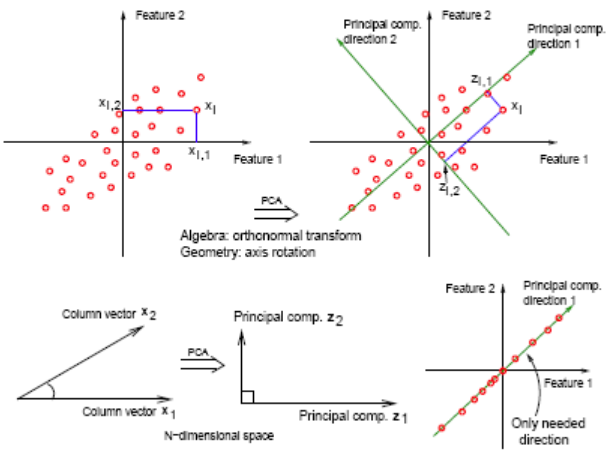
\includegraphics[height=7cm]{img/pc_directions_and_scores.png}
    %\caption{On a 2D basis, observation $\bxi = \begin{bmatrix}     x_{i1} & x_{i2}   \end{bmatrix}$ has projections (scores) $z_{i1}$ along $\bu_1$ and $z_{i2}$ along $\bu_2$. All $n$ observations get projected this way and the projections $\bz_1, \bz_2$ are uncorrelated.}
   \caption{Observation $\bxi = \left[x_{i1} \;\; x_{i2} \right]$ is projected on a 2D basis spanned by PC ``loadings'' $\bu_1,\ \bu_2$. The projected components along the basis vectors are $z_{i1}$ and $z_{i2}$ respectively. In the end, ``scores'' $\bz_1 = \left[z \right]$}
    
\end{figure}

We saw that to find each PC loading $\bu_j$ we rely on two important propertes -- the variance of the projection of all observations on each loading $\bu_j$ must be maximised and each PC score vector $\bz_j$ is uncorrelated to all previous ones. Exception is the first PC vector $\bz_1$ whose only requirement is that its variance is maximised. So we reach the following definition.
% ref https://www.ibmm.unibe.ch/unibe/portal/fak_naturwis/a_dept_math/a_dept_ms/content/e237483/e237655/e243381/e281679/files281689/Chap8-10_ger.pdf
% ref http://users.stat.umn.edu/~helwig/notes/pca-Notes.pdf

\begin{definition}[principal components]
\marginnote{\textup{Remember, the definition on the left holds assuming the features are in columns -- some authors stack them as rows so the product would become $\bu_j\t\bX$. The variance lemma remains the same though.}}
We define the principal components $\bu_1,\ldots,\bu_D$ such that:
\begin{align*}
    \textup{First\; PC\; } \bz_1 := &\textup{linear\; combination\;} \bu_1\t\bX \textup{\; that \; maximises\;}\sigma^2(\bX\bu_1)\\
    &\textup{s.t. \;} \bu_1\t\bu_1 = 1\\
    \textup{Second\; PC\;} \bz_2 := &\textup{linear\; combination\;} \bu_2\t\bX \textup{\; that \; maximises\;}\sigma^2(\bX\bu_2)\\
    &\textup{s.t. \;} \bu_2\t\bu_2 = 1 \textup{\; and \;} \sigma(\bX\bu_2, \bX\bu_1) = 0\\
    \vdots \\
    j\textup{-th\; PC\;} \bz_j := &\textup{linear\; combination\;} \bu_j\t\bX \textup{\; that \; maximises\;}\sigma^2(\bu_j\t\bX)\\
    &\textup{s.t. \;} \bu_j\t\bu_j = 1 \textup{\; and \;} \sigma(\bX\bu_j, \bX\bu_i) = 0 \quad \forall i < j\\
\end{align*}
\end{definition}
Before we derive how loading (direction) vectors must be chosen, it's important to note that the variance of each PC $\bz_j$ can be written as a prouduct involving the covariance matrix $\bSigma$.


\begin{lemma}[Variance along a PC in terms of covariance matrix]
\label{lem:var_wrt_cov_matrix}
The variance of centred data projected on a PC $\bu_j$, i.e. on $\bz_j = \bX\bu_j$ can be written as:
\begin{equation}
    \sigma^2(\bz_j) = \bu_j\t\boldsymbol{\Sigma}\bu_j
    \label{eq:pc_score_wrt_cov_matrix}
\end{equation}
% see http://jupiter.math.nctu.edu.tw/~yuhjye/assets/file/teaching/2017_machine_learning/PCAsubset.pdf
The covariance between score vectors $\bz_i, \bz_j$ can be written as:
\begin{equation}
	\sigma(\bz_i,\bz_j) = \bu_i\t\bSigma\bu_j = \bu_i\t\bSigma\bu_j
	\label{eq:pc_scores_cov_wrt_cov_matrix}
\end{equation}
	(since $\bSigma$ is symmetric).
\end{lemma}
\begin{proof}
	Recall that the data matrix $\bX$ contains the features as columns and the observations as row, therefore $\bX\t$ contains the observations as columns.

	Let's consider $\bz_j$. In \eqref{eq:pca_alg_form}, the $i$-th row $z_{ij}$ is the dot product $\bu_j\t\bX_i\t$, where $\bX_i\t$ is the $i$-th column of $\bX\t$, therefore the $i$-th observation vector. Then, $\bz_j$ can alternatively be written as:
	\[
		\begin{bmatrix}
			z_{1j} \\ z_{2j} \\ \vdots \\ z_{nj}	
		\end{bmatrix} = 
		\begin{bmatrix}
			\bu_j\t\bX_1\t	\\ \bu_j\t\bX_2\t	\\ \vdots \\ \bu_j\t\bX_n\t	\\
		\end{bmatrix}
	\]
	It's trivial to show that $\bz_j$ is zero-centred so its variance is simply the squared sum of its elements:
	\begin{align*}
	    \sigma^2(\bz_j) &= \frac{1}{n-1}\sum\limits_{i=1}^n{z_{ij}^2} \\
	    &= \frac{1}{n-1}\sum\limits_{i=1}^n(\bu_j\t\bX_i\t)(\bu_j\t\bX_i\t) \\
	    &= \frac{1}{n-1}\sum\limits_{i=1}^n \bu_j\t\bX_i\t\bX_i\bu_j  \tag*{($\ba\t\textbf{b}=\textbf{b}\t\ba$)}\\
	    &= \frac{1}{n-1}\bu_j\t\bX\t\bX\bu_j\\
	    & = \bu_j\t\bSigma\bu_j
	\end{align*}
	We can prove \eqref{eq:pc_scores_cov_wrt_cov_matrix} exactly the same way.
\end{proof}




\subsubsection{Deriving the first PC}

Given the data matrix $\bX$, we will see how $\bu_1$ must be chosen to satisfy the properties of the first PC loading, particularly to maximise $\sigma(\bz_1)$ subject to $\norm{\bu_1}=\bu_1\t\bu_1=1$. In \eqref{eq:pc_score_wrt_cov_matrix}, we also derived that $\sigma(\bz_1) = \sigma(\bX\bu_1) = \bu_1\t\bSigma\bu_1$, so we can prove the following.

\begin{corollary}[1st PC loading] 
The first PC loading $\bu_1$ is the eigenvector of the covariance matrix $\bSigma$ corresponding to its highest eigenvalue $\lambda_1$.
\label{cor:first_loading_eigenvec}
\end{corollary}
\begin{proof}
The first PC maximises $f(\bu_1)=\sigma_{\bX\bu_1} = \bu_1\t\bSigma\bu_1$ subject to $g(\bu_1) := \bu_1\t\bu_1 - 1 = 0$ so our constrained optimisation problem is:
\[
\max(\bu_1\t\boldsymbol{\Sigma}\bu_1) \quad \quad \quad \quad \textup{given} \;\; \bu_1\t\bu_1=1
\tag{1}
\label{eq:pc1_max_obj_function}
\]
% ref http://users.stat.umn.edu/~helwig/notes/pca-Notes.pdf
The $\bu_1$ that satisfies \eqref{eq:pc1_max_obj_function} can be found by introducing a Lagrange multiplier $\lambda$ such the Lagrangian cost function $\bL(\bu_1,\lambda) = f(\bu_1) - \lambda g(\bu_1)$ is maximised:
% ref http://jupiter.math.nctu.edu.tw/~yuhjye/assets/file/teaching/2017_machine_learning/PCAsubset.pdf
\begin{gather*}
\max\left(\bL(\bu_1,\lambda)\right) = \max\left(\bu_1\t\bSigma\bu_1 - \lambda(\bu_1\t\bu_1 - 1)\right) \Rightarrow\\
\frac{\partial f(\bu_1,\lambda)}{\partial \lambda} = 0 , \quad \frac{\partial f(\bu_1,\lambda)}{\partial \bu_1} = 0 \Rightarrow \\
\bu_1\t\bu_1 - 1 = 0  \label{eq:pc1_lagr_der1} \tag{2}  \\
\boldsymbol{\Sigma}\bu_1 - \lambda\bu_1 = (\Sigma - \lambda \textbf{I}_D)\bu_1 = 0  \label{eq:pc1_lagr_der2} \tag{3} 
\end{gather*}
Pre-multiplying the last equation by $\bu_1\t$ and using Lem. \ref{lem:var_wrt_cov_matrix} yields:
\begin{gather*}
  \bu_1\t\bSigma\bu_1 = \lambda\bu_1\t\bu_1 \Rightarrow\\
  \lambda = \sigma^2(\bz_1) \tag{4}
\end{gather*}

\eqref{eq:pc1_lagr_der1} and \eqref{eq:pc1_lagr_der2} tell us that the desired vector $\bu_1$ is an eigenvector of the covariance matrix $\Sigma$ and $\lambda$ is its first and largest eigenvalue.
\end{proof}



% - - - - - - - - - - - - - - - - - - - - - - - - - - - - - - - -
\subsection{Deriving the other PCs}

Before deriving the second PC loading, recall from Cor. \ref{cor:first_loading_eigenvec} that $\boldsymbol{\Sigma}\bu_1 = \lambda\bu_1$.
Next, we explore what zero correlation between two PC scores $\bz_i,\ \bz_j$ imposes on the  geometry of loadings $\bu_i,\ \bu_j$.
\begin{corollary}[orthonormal loading vectors] The loading vectors $\bu_1,\ldots,\bu_D$ form an orthonormal basis.
\label{cor:loading_vec_ortho}
\end{corollary}
\begin{proof}
We have already imposed that $\norm{\bu_j}=1$. Because of the eigenvector corollary, $\boldsymbol{\Sigma}\bu_1 = \lambda_1\bu_1$. Also, one of the properties is that $\sigma(\bz_i,\bz_j)=0$. Therefore, using \eqref{eq:pc_scores_cov_wrt_cov_matrix}:
% https://stats.stackexchange.com/questions/153928/why-are-principal-component-scores-uncorrelated?rq=1
\begin{align*}
\sigma(\bz_1,\bz_2) = &\bu_1\t\bSigma\bu_2 = \lambda_1\bu_1\t\bu_2 = 0 \Rightarrow\\
&\bu_1\t\bu_2=0
\end{align*}
We have shown the result for $\bu_2$ given $\bu_1$ but it holds for any $\bu_j$ given $\bu_i, \quad i < j$.
\end{proof}

% compare: https://www.ibmm.unibe.ch/unibe/portal/fak_naturwis/a_dept_math/a_dept_ms/content/e237483/e237655/e243381/e281679/files281689/Chap8-10_ger.pdf, https://online.stat.psu.edu/stat508/book/export/html/639, http://users.stat.umn.edu/~helwig/notes/pca-Notes.pdf

To derive the $j$-th PC loading $\bu_j$, we use the same variance maximisation property, however we add the fact that the current PC score it's uncorrelated to all previous PCs, i.e. $\sigma(\bz_i,\bz_j)=\sigma(\bX\bu_i, \bX\bu_j) = 0 \quad \forall \i < j$. Recall from \eqref{eq:pc_scores_cov_wrt_cov_matrix} that $\sigma(\bX\bu_i,\bX\bu_j) = \bu_i\t\bSigma\bu_j$ and that covariance needs to be zero. We will show how $\bu_2$ is computed given $\bu_1$.
% see https://www.cs.princeton.edu/courses/archive/fall18/cos324/files/pca.pdf
% ref
\begin{gather*}
    \max(\bu_2\t\boldsymbol{\Sigma}\bu_2) \\
    \textup{given} \;\; \bu_2\t\bu_2=1 \\
	\textup{and} \;\; \bu_1\t\bSigma\bu_2 = 0
\end{gather*}
However, we deduced that $\bu_1\t\bSigma\bu_2 = 0$ implies $\bu_1\t\bu_2 = 0$. Therefore if $\lambda,\mu$ the Lagrange multipliers, the Lagrange multiplier we want to maximise it:
% http://jupiter.math.nctu.edu.tw/~yuhjye/assets/file/teaching/2017_machine_learning/PCAsubset.pdf
% http://www.bbk.ac.uk/ems/faculty/brooms/teaching/SMDA/SMDA-02.pdf
\[
\mathcal{L}(\bu_1,\bu_2) = \bu_2\t\bSigma\bu_2 - \lambda\bu_2\t\bu_2 - \mu\bu_2\t\bu_1 = 0
\]
% ref https://courses.cs.ut.ee/MTAT.03.227/2014_spring/uploads/Main/lecture-notes-9.pdf
Differentiate w.r.t. $\bu_2$ and set the derivative to zero:
\[
\frac{\partial \mathcal{L}}{\partial \bu_2} = 0 \Rightarrow \bSigma\bu_2 - \lambda\bu_2 - \mu\bu_1 = 0 \tag{4}
\label{eq:lagr_cond_pc2}
\]
Pre-multiply by $\bu_1$
\[
\bu_1\t\bSigma\bu_2 - \lambda\bu_1\t\bu_2-\mu\bu_1\t\bu_1 = 0 \Rightarrow \mu = 0 
\]
,since $\sigma(\bz_1,\bz_2)= \bu_1\t\bSigma\bu_2=0$ (\eqref{eq:pc_scores_cov_wrt_cov_matrix} and property 3), $\bu_1\t\bu_2=0$ (Cor. \ref{cor:loading_vec_ortho}) and $\bu_1\t\bu_1=1$. Plugging in $\mu=0$ back in \eqref{eq:lagr_cond_pc2}, we find exactly that $\lambda$ is an eigenvalue  $\lambda_2$ of $\bSigma$ corresponding to eigenvector $\bu_2$:
\begin{gather*}
    \bSigma \bu_2 = \lambda_2\bu_2 \Rightarrow \\
    \bu_2\t\bSigma \bu_2 = \lambda_2\bu_2\t\bu_2 \Rightarrow\\
    \lambda_2 = \sigma^2({\bz_2})
\end{gather*}
% ref % http://www.bbk.ac.uk/ems/faculty/brooms/teaching/SMDA/SMDA-02.pdf
Recall also that $\lambda \neq \lambda_1$ and $\lambda_1 \geq \lambda_2$ due to property 2 of PCs. Similarly we derive:
\begin{gather*}
    \bSigma\bu_j = \lambda_j \bu_j, \quad \lambda_j = \sigma^2(\bz_j) \\
        \bSigma\bu_{j+1} = \lambda_{j+1} \bu_{j+1}, \quad \lambda_{j+1} = \sigma^2(\bz_{j+1}) \\ 
        \ldots \\
         \bSigma\bu_D = \lambda_D \bu_D, \quad \lambda_D = \sigma^2(\bz_D)
\end{gather*}
The eigenvectors $\bu_j$ corresponding to each eigenvalue $\lambda_j$ are arranged in descending order, i.e. $\lambda_j \geq \lambda_{j+1}$ since $\lambda_j = \sigma^2(\bz_j)$ and due to property 2. We have arrived at the following conclusion.
\begin{lemma}[how each PC is computed given the data matrix]
Given a data matrix $\bX_{n\times D}$, where $n$ is the number of observations and $D$ the features (dimensions) of each one, then each PC loading (direction of the projection data) is the $j$-th eigenvalue of the covariance matrix $\bSigma$, i.e.
\begin{equation}
    \bSigma\bu_j = \lambda_j\bu_j
\end{equation}
THe $j$-th eigenvalue is the variance of the data projected on loading $\bu_j$, i.e. the variance of vector $\bz_j$:
\begin{equation}
    \lambda_j = \sigma^2(\bz_j) = \sigma^2(\bX\bu_j)
    \label{eq:var_as_eigenval}
\end{equation}
\end{lemma}
The variance expresses how much information each direction $\bu_j$ ``holds'', i.e. its significance. So when we perform PCA we can only keep the first $d$ components based on their total relative significance $\sum_{i=1}^d\lambda_i/\sum_{i=1}^D\lambda_i$.


\subsubsection{The relative significance of the first $d$ components}
\label{sec:significance_first_k_comps}
When we want to project the original $D$ dimensional data to a  $d$-dimensional space, $d\leq D$, then due to \eqref{eq:var_as_eigenval} the part of variance explained by the first $d$ PCs is:
\begin{equation}
    R = \frac{\sum\limits_{i=1}^d \sigma^2(\bz_i)}{\sum\limits_{i=1}^D \sigma^2(\bz_i)} = \frac{\sum\limits_{i=1}^d\lambda_i}{\sum\limits_{i=1}^D \lambda_i}
\end{equation}
, where $\lambda_i$, $\lambda_1 \geq \lambda_2 \geq \ldots \geq \lambda_D$ are the eigenvalues of the covariance matrix $\bSigma$  after we centred our data, i.e. the mean of each feature (column) of $\bX$ is zero. 

There are two common rules of thumb to select $d$.
\begin{enumerate}
    \item Require the variance explained by the first $d$ components to be equal at least to a percentage $r$. Then we simply choose the minimum integer $d$ such that:
    \[
    d=\arg \min\left(100\sum\limits_{i=1}^d\lambda_i/\sum\limits_{i=1}^D \lambda_i\right) \geq r, \quad 0 < r < 100 
    \]
    \item Find the ``elbow'' of the \emphasis{scree plot}. The scree plot is simply the (discrete) plot of the value of each eigenvalue $\lambda_1,\ldots,\lambda_D$ on the $y$-axis against their index $i$ on the x-axis. The elbow is the index of what it looks like the inflexion point of that plot, i.e. index before the plot starts to flatten. The contribution of the eigenvalues beyond the elbow is considered insignificant. An example is illustrated below.
    % ref http://www.cs.cmu.edu/~mgormley/courses/606-607-f18/slides606/lecture11-pca.pdf
    \begin{figure}[H]
        \centering
        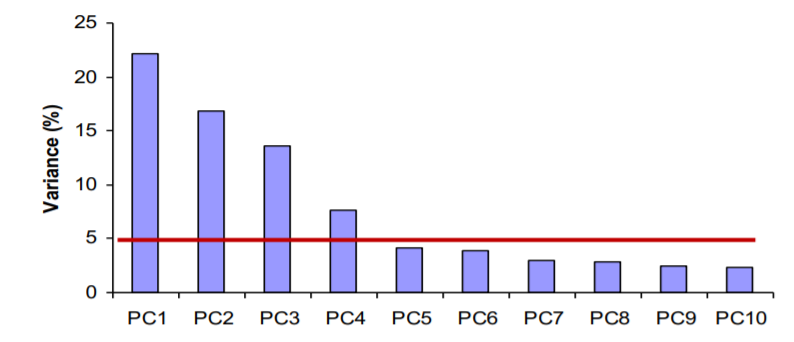
\includegraphics[height=4.5cm]{img/scree_plot.PNG}
        \caption{Scree plot of some hypothetical 10-dimensional data. In this case, we could choose $i=4$ as the elbow, ignoring the contributions of $PC_5,\ldots,PC_{10}$.}
        \label{fig:my_label}
    \end{figure}
\end{enumerate}


\subsubsection{Reconstruction of the original data}
% ref https://stats.stackexchange.com/questions/229092/how-to-reverse-pca-and-reconstruct-original-variables-from-several-principal-com
Sometimes it's useful to reconstruct the original non-centred data $\bX$ given the PC scores $\bz_1,\ldots,\bz_D$. To see how, re-write \eqref{eq:pc_score_as_product_compact} by setting $\bX_c$ as $\bX$, to make it clear that is denoted the centred data. Also set $\textbf{Z} := \begin{bmatrix} \bz_1 & \ldots & \bz_D\end{bmatrix}$, $\textbf{U} := \begin{bmatrix} \bu_1 & \ldots & \bu_D\end{bmatrix}$. As a reminder, $\textbf{U}$ stores the eigenvectors of $\bSigma$ in descending order. Then:
\begin{gather}
    \textbf{Z} = \bX_c \textbf{U}\Rightarrow \nonumber \\
    \bX_c = \textbf{Z} \textbf{U}\t \nonumber
\end{gather}
We obtain the approximation $\hat{\bX}$ of the original data by adding its mean to each column of $\bX_c$:
\begin{equation}
    \hat{\bX} = \bX_c + \bar{\bX} = \textbf{Z} \textbf{U}\t + \bar{\bX}, \quad \bar{\bX} = 
    \begin{bmatrix}
    | & | & | \\
    \bar{\bx_1} & \ldots & \bar{\bx_D} \\
    | & | & |
    \end{bmatrix}
\end{equation}
If we use all $D$ basis vectors, like above, the error $\norm{\hat{\bX} - \bX}^2$ should be very close to zero (practically it's not exactly zero due to floating point). If we perform a lossy reconstruction, i.e. use $d < D$ componenents, then we can discard the $D-d$ last columns of $\textbf{U}$, and the last $D-d$ columns of $\textbf{Z}$ (but we don't discard columns of $\bX_c$, notice the product size is still $n\times D$):
\begin{equation}
    \hat{\bX} = \bX_c + \begin{bmatrix}
    \bz_1 & \ldots & \bz_d
    \end{bmatrix}\begin{bmatrix}
    \bu_1 & \ldots & \bu_d
    \end{bmatrix}\t
    \label{eq:recon_non_centred_data}
\end{equation}
As we saw in the next section, the information retention of the first $d$ components is $\sum\limits_{i=1}^d \lambda_i/\sum\limits_{i=1}^D \lambda_i$. The larger the better but at the same time the more components, the larger the dimensionality of the projected data, which is a undesired. The basics of PCA have been presented and in the next section there is a summary of the algorithm.
% https://www.quora.com/How-does-PCA-maximize-projected-variance-through-the-covariance-matrix



\subsection{Data pre-processing -- feature whitening}

The essential steps of PCA have been presented, but in real world one more  pre-processing step, called whitening is often required. In practice, data contained in the rows of $\bX$ might have different scales by one or more orders of magnitude or may be highly correlated. The aim of what's called \emphasis{whitening} is
% ref http://ufldl.stanford.edu/tutorial/unsupervised/PCAWhitening/
\begin{enumerate}
    \item to make the features are less correlated with each other
    \item and to make all features have the same variance.
\end{enumerate}
\marginnote{Whitening is recommended when features have different orders of magnitude.}Aim 1 is addressed by the covariance of two scores being zero so it's already achieved in PCA. The problem when we have a data matrix where one feature $\bx_1 \approx 10^3 \bx_2$, then for the the eigenvalue of $\bSigma$ we'd have $\lambda_1 >> \lambda_2$, so feature $\bx_1$ when projected to loading 1, $\bx_1\t\bu_1$, will capture most of the significance just because its values are large. Whitening alleviates this.
\begin{definition}[feature whitening]
Whitening a feature $\bx_j$ sets its mean to zero and its variance to unit and is expressed by:
\begin{equation}
    \bx_{j,white} = \frac{\bx_j - \bar{\bx_j}}{\sigma_{\bx_j}},\quad \bar{\bx_j} = \textbf{1}_n\sum\limits_{i=1}^n \frac{\bX_{ij}}{n}
    \label{eq:data_whiten}
\end{equation}
\end{definition}
In our case, we assume that $ \bar{\bx_j}$ since we always centre the data as soon as we obtain it. So then $\sigma^2_{\bx_{j,white}} = \sum\limits^n x_{ij}^2/\sigma_{\bx_j} = \sigma^2_{\bx_j}/\sigma^2_{\bx_j} = 1$.


\subsection{The PCA algorithm}
We summarise the steps to obtain the PCA of a data matrix $\bX$, assuming $\bX$ stores the observations are rows.

\begin{enumerate}
    \item Centre the features of the data matrix using \eqref{eq:centred_matrix_wrt_original} to obtain matrix $\bX_c$. Optionally, if the features have different orders of magnitiude, whiten them using \eqref{eq:data_whiten}.
    \item Compute the covariance matrix $\bSigma = \bX_c\t\bX_c$.
    \item Find the first $d$ eigenvectors of $\bSigma$ with largest eigenvalues $\bu_1,\ldots,\bu_d$; we called those ``loadings''.
    \item Find the projections $\bz_1 = \bX_C\bu_1,\ \bz_2 = \bX_C\bu_2,\ \ldots, \ \bz_d = \bX_C\bu_d$. These are called ``scores'' and they approximate the centred set, but spanned by the basis $\bu_1,\ldots,\bu_d$. PCA returns the loads, scores, and the corresponding eigenvalues of the scores. 
\end{enumerate}

Let's verify the algorithm and the formulas for the PCs in Matlab. We'll be using Matlab's (not available in Octave) \texttt{pca} function to get the correct results and the eigendata (\texttt{eigs}) to follow the algorithm. For reference, the return of these two function is the following:
\begin{minted}[style=code1]{matlab}
% X is n by D, i.e. observations are stacked as rows
[loads, pcs, pca_eval] = pca(X)
% V is the matrix with eigenvectors as columns,
% D diagonal with eigenvalues in descending order 
[V,D] = eigs(A)
\end{minted}
\begin{enumerate}
    \item (\textit{Create some data}) We'll be using some synthesised data whose each ovservation contains a weight, height, and IQ $(w, h, iq)$. We'll create the data such that the weight is positively correlated with height and IQ is independent of both. The data consist of 1000 observations.
    \begin{minted}[style=code1]{matlab}
    h = random('norm', 177, 5, 1000, 1);
    w = h/2 - 15 + 10*random('uniform', 0, 1, 1000, 1);
    iq = random('norm', 105, 10, 1000, 1);
    X = [w, h, iq];
    » X
    ans =
        80.8160  179.8088   87.1759
        83.8719  179.7486  104.0231
        84.5937  188.9917  106.7827
        79.9716  179.2866  105.9784
        83.1234  180.2754  121.5708
        78.5173  173.9326  106.1138
        78.0839  176.9065  121.0178
        <-- omitted -->
    \end{minted}
    \item (\textit{Calculate covariance matrix}) Centre the data using \eqref{eq:centred_matrix_wrt_original} and then calculate $\bSigma$.
    \begin{minted}[style=code1]{matlab}
    n = size(X,1);
    C = eye(n) - 1/n*ones(n,1)*ones(n,1)';
    Xc = C*X;
    S = Xc'*Xc;
    » S
        S =
        1.0e+04 *
        1.4384    1.1808    0.0451
        1.1808    2.2948   -0.1340
        0.0451   -0.1340    9.3945
    \end{minted}
    
    \item (\textit{Find the eigenvalues of covariance matrix}) Recall the \texttt{eigs} command and what it returns. Eigenvectors of $\bSigma$ are our loading vectors $\bu_1,\bu_2,\bu_3$. We can also verify that their dot products are zero.
    \begin{minted}[style=code1]{matlab}
    [evec,eval] = eigs(S);
    u1 = evec(:,1); u2 = evec(:,2); u3 = evec(:,3);
    » u1' * u2
    ans =
        -6.9389e-18
    \end{minted}
    \item (\textit{Compute and verify and PC scores}) Use \eqref{eq:pc_score_as_product}. Compare against \texttt{pca}'s values.
    \begin{minted}[style=code1]{matlab}
    z1 = Xc*u1; z2 = Xc*u2; z3 = Xc*u3;     
    [loads, pcs, pca_evals] = pca(Xc);
    » loads
        loads =
        0.0029    0.5745    0.8185
       -0.0184    0.8184   -0.5744
        0.9998    0.0133   -0.0130
    » evec
        evec =
        0.0029    0.5745   -0.8185
       -0.0184    0.8184    0.5744
        0.9998    0.0133    0.0130
    % 3rd eigenvector is flipped but it doesn't matter as they specify direction
    » pcs - [z1 z2 z3]
        ans =
        -0.3908   -0.0888    0.1776
        -0.4263   -0.1066    0.2132
        -0.3908   -0.1243    0.1732
        -0.4041   -0.1599    0.2021
        -0.4241   -0.0910    0.1954
        <-- omitted -->
    \end{minted}
    The difference between the PCs scores from scratch (\texttt{z1, z2, z3}) and Matlab's scores is small but not exactly zero, possibly due to implementation discrepancies (?).
    \item (\textit{Reconstruct the original data}) Use \eqref{eq:recon_non_centred_data}. First we'll reconstruct the original using the full basis $\{\bu_1,\bu_2,\bu_3 \}$ (matrices $\textbf{U}_3,\textbf{Z}_3$) and then using $\{\bu_1,\bu_2\}$ (matrices $\textbf{U}_2,\textbf{Z}_2$).  
    \begin{minted}[style=code1]{matlab}
    U3 = [u1 u2 u3]; U2 = [u1 u2];
    Z3 = [z1 z2 z3]; Z2 = [z1 z2];
    X_recon_3 = Z3*U3' +...
        [mean(X(:,1))*ones(n,1), mean(X(:,2))*ones(n,1), mean(X(:,3))*ones(n,1)];
    X_recon_2 = Z2*U2' +...
        [mean(X(:,1))*ones(n,1), mean(X(:,2))*ones(n,1), mean(X(:,3))*ones(n,1)];
    » X_recon_3 - X
        ans =
        0.0853    0.2842    0.0995
        0.0995    0.2558    0.1421
        0.0995    0.2558    0.1137
        0.0853    0.2558    0.1137
        0.0853    0.2558    0.1137
        <-- omitted -->
    » norm(X_recon_3 - X, 2)
        ans =
        8.6679e-12
    » norm(X_recon_2 - X, 2)
        ans =
        78.0468
    \end{minted}
\end{enumerate}
From the last answer, we can see that $\textbf{U}_3$ reconstructs better the original data than $\textbf{U}_2$. The three figures below visualise the loadings $\bu_1,\bu_2,\bu_3$ and the centred data cloud. Notice how each loading captures the maximum variation of the data and how they are mutually orthogonal. Loadings have been exaggerated by 20 times so that they are visible.
\begin{multicols}{3}
  \begin{figure}[H]
      \centering
      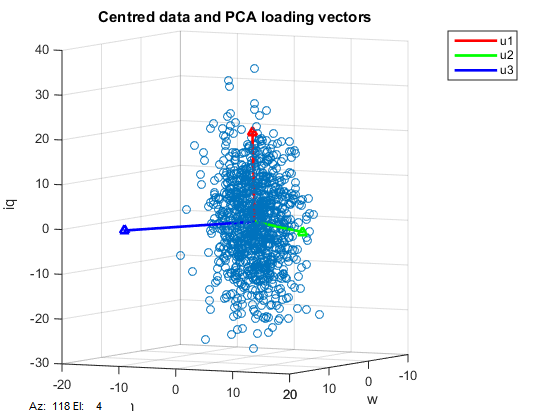
\includegraphics[width=0.33\textwidth]{img/whiq_xyz.png}
      \caption{The centred data and loadings in 3D.}
  \end{figure}
  
 \columnbreak
   \begin{figure}[H]
      \centering
      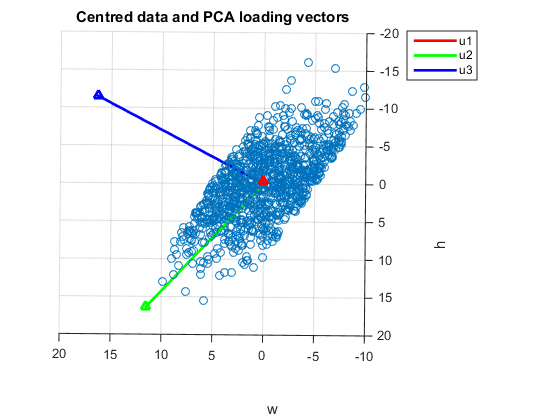
\includegraphics[width=0.33\textwidth]{img/whiq_xy.png}
      \caption{The data and loadings in the $x_1,x_2$ plane.}
  \end{figure}
 
 \columnbreak
   
 \columnbreak
   \begin{figure}[H]
      \centering
      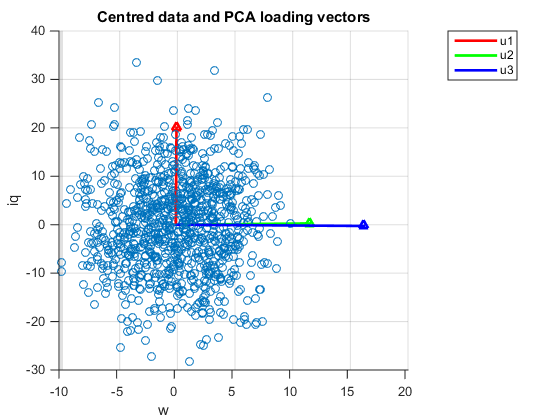
\includegraphics[width=0.33\textwidth]{img/whiq_xz.png}
      \caption{The data and loadings in the $x_1,x_3$ plane.}
  \end{figure}
\end{multicols}
The above steps are generalised in the Matlab function \texttt{my\_pca}, found in \ref{app:my_pca_matlab}. 
  

% https://alliance.seas.upenn.edu/~cis520/wiki/index.php?n=Lectures.PCA
% https://shreydesai.github.io/2019/02/14/principal_component_analysis.html
% 
% https://en.wikipedia.org/wiki/Principal_component_analysis#Calculate_the_empirical_mean

\subsubsection{PCA via SVD}

SVD (Singular value decomposition) is a method of decomposing a any matrix $\bX_{n\times d}$ three matrices $\textbf{U}, \textbf{D}, \textbf{V}$. It's very powerful and used in numerous applications. SVD is available in many libraries and frameworks and can help quickly compute the PCA essentially out of the box.
\begin{theorem}[SVD]
Any matrix $\bX_{n\times d}$ can be written as a product of two orthogonal matrices $\textbf{U},\textbf{V}$ and a diagonal one $\textbf{D}$.
\begin{equation}
    \bX = \textbf{U}\textbf{D}\textbf{V}\t
\end{equation}
\begin{itemize}
    \item $\textbf{V}_{n\times D}$ contains the eigenvectors of $\bX'\bX$ as columns. They are arranged from the one that corresponds to the one that corresponds to the largest eigenvalue to one that corresponds to the smallest.
    \item $\textbf{D}$ A diagonal matrix that contains the \emphasis{singular values} of $\bX$ in descending order, i.e. the square roots of the eigenvalues of $\bX\t\bX$:
    \begin{equation}
        \textbf{D} =
        \begin{bmatrix}
        \sqrt{\lambda_1(\bX\t\bX)} & & \\
         & \ddots & \\
         & & \sqrt{\lambda_D(\bX\t\bX)}
        \end{bmatrix}, \quad \lambda_1(\bX\t\bX) \geq \ldots \geq \lambda_D(\bX\t\bX)
    \end{equation}
    \item $\textbf{U}_{n\times D}$: 
    \begin{equation}
        \textbf{U} = \begin{bmatrix}
        | & | & | \\
        \frac{\bX\bu_1}{\norm{\bX\bu_1}} & \ldots & \frac{\bX\bu_D}{\norm{\bX\bu_D}}\\ 
        | & | & | 
        \end{bmatrix}
    \end{equation}
\end{itemize}
\end{theorem}
Again, the assumption is that $\bX$ has its columns centred. Then $\bX\t\bX$ is the covariance matrix, and SVD computes its eigenvalues in $\textbf{V}$, so the ``loads'' of PCA. Next, we simply compute the ``scores'' from \eqref{eq:pc_score_as_product_compact} as:
\begin{equation}
    \textbf{Z} = \bX\textbf{V}
\end{equation}
Alternatively, notice the $\textbf{U}$ matrix already contains the scores as unit vectors so each score $\bz_i$ can be obtained as:
\begin{equation}
    \bz_i = \textbf{u}_i \norm{\bX\textbf{v}_i}
\end{equation}
Finally, we can keep the first $d$ scores (columns) of $\textbf{U}$ to retain the most useful information.

% cont here: https://courses.cs.ut.ee/MTAT.03.227/2014_spring/uploads/Main/lecture-notes-9.pdf
% http://www.bbk.ac.uk/ems/faculty/brooms/teaching/SMDA/SMDA-02.pdf
% https://www.coursera.org/lecture/machine-learning/principal-component-analysis-algorithm-ZYIPa
% https://www.machinelearningplus.com/machine-learning/principal-components-analysis-pca-better-explained/
% https://www.edureka.co/blog/principal-component-analysis/
% https://towardsdatascience.com/principal-component-analysis-for-dimensionality-reduction-115a3d157bad


\subsection{Interpreting and visualising PCA results}

As defined before, each loading has the same size as an observation, i.e. $\bu\in \setR^{d}$. For instance, after performing PCA on a 3-feature dataset, we could have:
\begin{gather*}
\bu_1 = \begin{bmatrix}
0.36  \\ 0.91  \\ 0.18
\end{bmatrix} = 
0.36\begin{bmatrix}
1 \\ 0 \\ 0
\end{bmatrix} +
0.91\begin{bmatrix}
0 \\ 1 \\ 0
\end{bmatrix}+
0.18\begin{bmatrix}
0 \\ 0 \\ 1
\end{bmatrix} = 0.36\textbf{e}_1+0.91\textbf{e}_2+0.18\textbf{e}_3, \\
\bu_2 = \begin{bmatrix}
  -0.91 \\  0.36  \\ 0
\end{bmatrix}
\end{gather*}
Therefore if our dataset consisted of e.g. weight, height, IQ measurements, the above equation would imply that feature 2 (height) carries the most information (variance)/ When we looked at an observation, its height would be the most ``interesting'' feature as it would carry most of the information, followed by its weight, followed by its IQ. $\textbf{u}_2$ mostly conveys the weight.

\marginnote{Keep 2 PCs $\rightarrow$ plot in 2D.}Let's say that we want to approximate all measurements given the two first loadings $\textbf{u}_1,\textbf{u}_2$. Each score can be written as $\bz_i = w_1\bu_1 + w_2\bu_2$, where $w_1,w_2$ some weights. If we were to plot $\bz_1$ in 2D (since it's approximated by 2 loadings), we would plot point $(w_1,w_2)$ in Cartesian coordinates.

\subsection{Application 1. Analysing wine data.}

The wine dataset by UCI is used, which contains 178 wine measurements, each one with 13 attributes, such as alcohol percentage, hue, etc. The dataset is found in file \texttt{wine\_data.csv} as is adapted from the one at: \url{https://github.com/anishagartia/PCA-of-Wine-Dataset} to contain a header with the feature names. The original file contains also the class in the first column but that column has been removed. The exact same dataset can be loaded as:
\begin{minted}{python}
from sklearn.datasets import load_wine
# ...
X = load_wine()
\end{minted}
in Python, but we want to file to be passed as an argument instead.

A PCA wrapper which includes all the mandatory steps, as well as the optional (whitening) has been written at \texttt{wines/my\_pca.py}. To run it, execute file \texttt{wines/run\_my\_pca.py} with the following arguments:
\begin{verbatim}
python run_my_pca.py dataset_csv n_pc_components_to_keep 0|1
\end{verbatim}
, where 1 plots the first 2 PCs in 2D and 0 doesn't and \texttt{n\_pc\_components\_to\_keep} is an integer. The source is found in \ref{app:wine_src_code}. Running it, we obtain the following results. Note the 2D visualisation is very similar to the one in \texttt{sklearn}'s documentation page \footnote{\url{https://scikit-learn.org/stable/auto_examples/preprocessing/plot_scaling_importance.html\#sphx-glr-auto-examples-preprocessing-plot-scaling-importance-py}}. It's not exactly the same as the documentation splits the dataset in testing and training data and follows a slightly different pipeline.
\begin{figure}[H]
    \centering
    \captionsetup{width=.45\linewidth}
    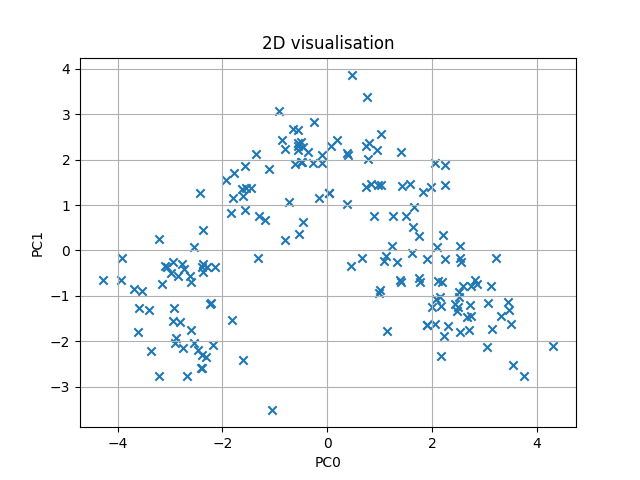
\includegraphics[width=.4\linewidth]{img/wine_result_2d.png}
    \caption{The scores of the first 2 PCs for all wines. PC0 mainly depends on, flavanoids (see below) and for PC1 on colour intensity.}
\end{figure}
Regarding the most important features, the following are printed if we keep the first 3:
\begin{verbatim}
The most important attributes are:
Flavanoids,Color_intensity,Ash
\end{verbatim}


\subsection{Application 2. Eigenfaces.}

Eigenfaces is a method that uses PCA to recognise faces. It is essentially PCA with \textit{pixels as features}. It employs a face database, which stores various face images of various subjects (e.g. 8 images of each person). When a novel face is detected, it finds its closest match in the database and outputs the subject number. If the novel face does not belong to any of the subjects, it is added to the database.
\begin{figure}[H]
    \centering
    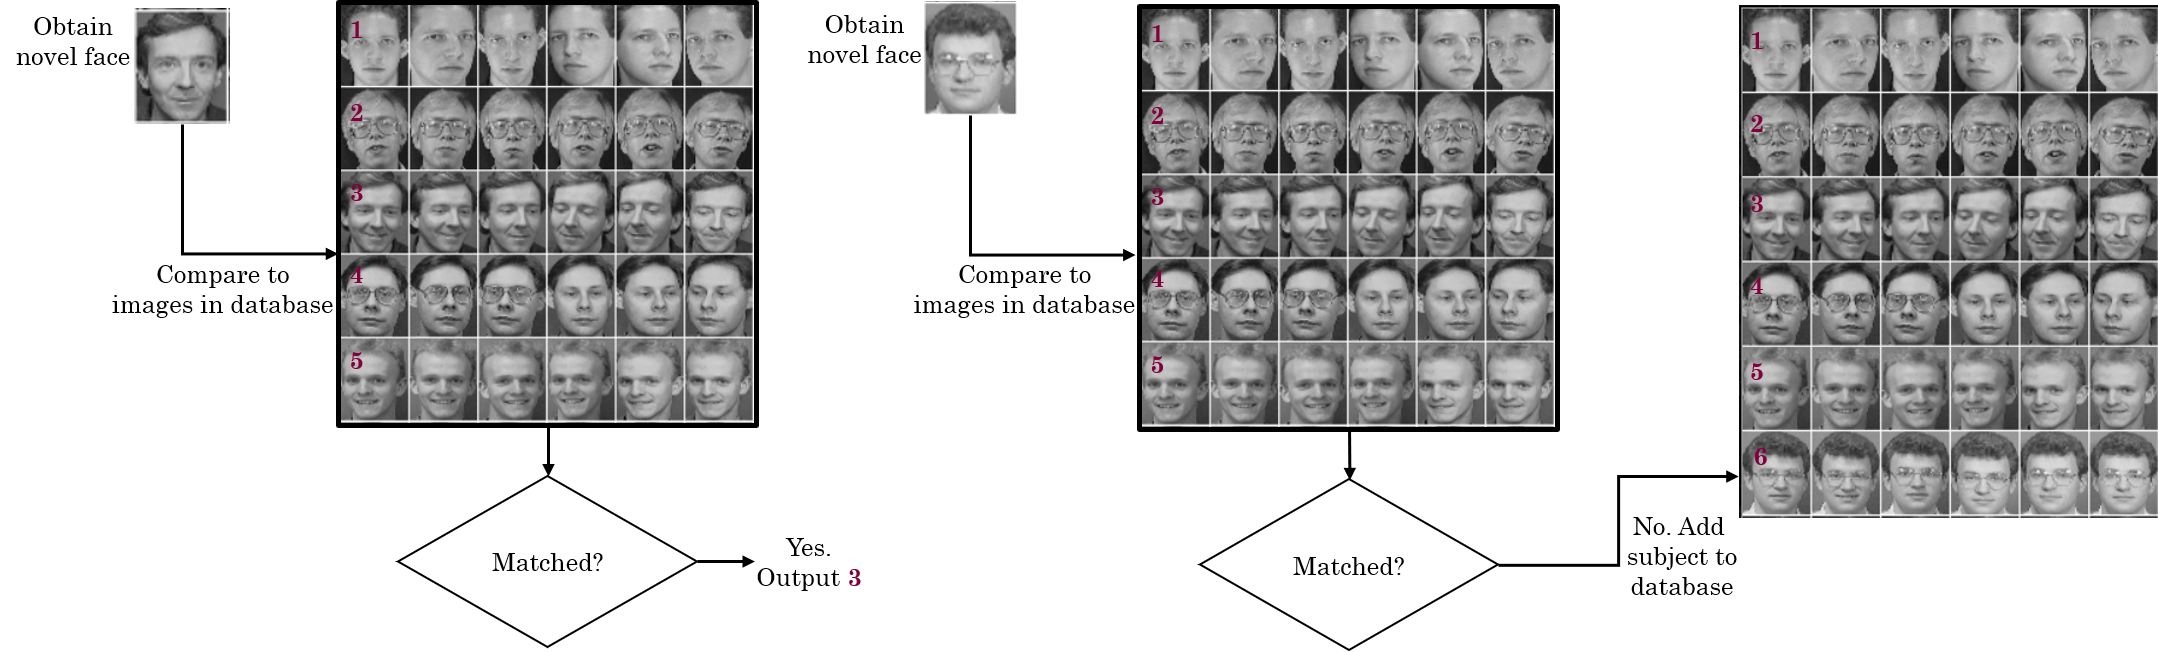
\includegraphics[width=\linewidth]{img/matching_face_to_db.png}
    \caption{Face recognition takes a new face as input and finds its best match in the database. Each row corresponds to a subject's stored faces, labelled with an integer.}
\end{figure}
The main question to answer in order to figure out how Eigenfaces work is ``\textit{how is matching accomplished?}''. Before matching is performed, it requires that each face in the database and the novel face (the new face, the one we try to match) are all represented by their coordinates in a new orthonormal subspace instead of as pixel ({training phase}). Next, by comparing the distance between the coordinates of a novel face with those of the stored faces, matching is accomplished ({prediction phase}). Below are the steps for the training phase.

% http://vision.stanford.edu/teaching/cs131_fall1415/lectures/lecture17_face_recognition_cs131.pdf
% http://vision.jhu.edu/teaching/vision08/Handouts/case_study_pca1.pdf
% https://www.cs.cornell.edu/courses/cs4786/2016sp/lectures/lec03.pdf
% https://jeremykun.com/2011/07/27/eigenfaces/
% https://pythonmachinelearning.pro/face-recognition-with-eigenfaces/
\begin{enumerate}
	\item (\textit{Compile the database}) Gather $M$ face images. Each image must be labelled with the subject's number.
	Convert them to greyscale and resize them all to the same shape, e.g. $N\times N$. Flatten each image row by row and store it in a row vector $\bX_i \in \setR^{N\times N}$.
			Stack those vectors horizontally to form the data matrix $\bX$ of size $M\times N^2$:
			\begin{equation}
				\bX = 
				\begin{bmatrix}
					- & \bX_1 & - \\	
					- & \bX_2 & - \\	
					 & \ldots & \\
					- & \bX_M & - \\	
				\end{bmatrix}, \quad \bX_i \in \setR^{1\times N^2}
			\end{equation}
		
\item (\textit{Centre the features by subtracting the mean image}) PCA is applied on data with zero-mean features. The features of the dataset are in this case all pixels at positions $1,2\ldots,N^2$ (columns of matrix $\bX$) over all $M$ faces. Therefore each feature (pixel) $\bX_i\in \setR^M$ will have its mean $\bu_i$ subtracted from it (mean over all $M$ images). The centred matrix $\bX_c$ is defined as:
	\[
		\bX_c =  \begin{bmatrix}
			| & | &  & | \\
			\bX_1 -	\boldsymbol{\mu}_1 & \bX_2 -	\boldsymbol{\mu}_2 &\ldots &\bX_{N^2} -	\boldsymbol{\mu}_{N^2} &\\
			| & | &  & | 
		\end{bmatrix} = \bX - \textbf{1}_{M\times 1}\boldsymbol{\mu}\t, \quad
		\boldsymbol{\mu} = \frac{1}{M} \bX\t \textbf{1}_{M\times 1}, \quad \boldsymbol{\mu}\in\setR^{N^2}
	\]
	From \eqref{eq:centred_matrix_wrt_original}, we know that we can rewrite the above equation to obtain the centred data matrix $X_c$ through a single matrix multiplication as:
		\begin{equation}
			\bX_c = \bC\cdot \bX, \quad \bC = \textbf{I}_M - \frac{1}{M}\textbf{1}_{M\times 1}\textbf{1}_{M\times 1}\t 
		\end{equation}
		, where $\textbf{1}_{M\times 1}$ contains only ones. Visually, subtracting the mean matrix gets rid of all the genetic features of each face and keeps the prominent ones (nose, lips, etc.). 

		\begin{multicols}{3}
			\begin{figure}[H]
				\centering
				
\includegraphics[width=0.25\linewidth]{img/eigfaces_sample.png}
				\caption{First sample $\bX_1$ of the Olivetti faces dataset.}
				\label{fig:eigfaces_samples}
			\end{figure}
		\columnbreak	

			\begin{figure}[H]
				\centering
				
\includegraphics[width=0.25\linewidth]{img/eigfaces_means.png}
				\caption{The mean image $\boldsymbol{\mu}$ of Oliveti dataset images.}
				\label{fig:eigfaces_samples}
			\end{figure}
		\columnbreak

			\begin{figure}[H]
				\centering
				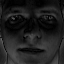
\includegraphics[width=0.25\linewidth]{img/eigfaces_diff.png}
				\caption{The absolute value of the same sample after the mean is subtracted from it $\left|\bX_1-\boldsymbol{\mu}\right|$.}
				\label{fig:eigfaces_diff}
			\end{figure}
		\end{multicols}
	\item (\textit{Compute the eigenvectors of the covariance matrix of $\bX_c$, $\boldsymbol{\Sigma} = \bX_c\t\bX_c$}) Recall that matrix $\bX_c$ is of size $M\times N^2$ so $\bSigma = \bX_c\t\bX_c$ is of size $N^2\times N^2$. If the original images were of size $64\times 64$, then $\bSigma\in \setR^{3844\times 3844}$, which is too huge to perform eigen-analysis!

		From Lemma \ref{lem:eig_ata_aat}, recall that if we know the eigen-data $\mu_i, \textbf{v}_i$ of $\bX_c\bX_c\t$, then the eigen-data $\lambda_i, \bu_i$ of $\bX_c\t\bX$ are given by:
		\begin{align}
			\lambda_i = \bu_i, & & & \bu_i = \bX_c\t\textbf{v}_i	
			\label{eq:eif_of_XTX_given_XXT}
		\end{align}
		The eigenvectors of $\bSigma = \bX_c\t\bX_c$ are called \emphasis{eigenfaces} and the space the $K$ first eigenvectors span, i.e. $\{\bu_1,\ldots,\bu_K\}$ is called \emphasis{face space}.  
	\item(\textit{Compute the eigenface space representation of each image})
Now since $\bu_i$ form an orthonormal space, each face $\bX_i$ can be represented as their linear combination, or $\bX_i = w_{i1}\bu_1 + \ldots + w_{iM}\bu_M = \textbf{w}_i\t \begin{bmatrix}
	\bu_1 & \bu_2 & \ldots & \bu_M	
\end{bmatrix}$. And since we want to keep only the first $K$ eigenvectors\footnote{The number $K$ can be determined by comparing the relative significance of the first $K$ eigenvectors to a threshold, e.g. 0.9. The relative significance was derived in section \ref{sec:significance_first_k_comps}.}, we can approximate $\bX_i$ as the linear combination of $w_{i1}\bu_1 + \ldots + w_{iK}\bu_K$. Then each $j$-th coefficient that describes face $i$, i.e. $w_{ij}$, is computed by the inner product $w_{ij} = \bX_i\t\bu_j$. For instance, for face 1, $w_{11} = \bX_1\t\bu_1$, $w_{12} = \bX_1\t\bu_2,\ldots w_{1K} = \bX_1\t\bu_K$. Similarly, we can find the coefficients $w_{2i}$ of face $\bX_2$. More compactly, the coordinates of each face can be computed as the matrix rows of $\textbf{W}$:
\begin{equation}
	\textbf{W}_i = \bX_i \cdot \textbf{U}, \quad
		\textbf{U}= \begin{bmatrix}
		\bu_1 & \ldots & \bu_K	
	\end{bmatrix}	
	\label{eq:eigenface_coords_matrix}
\end{equation}
\end{enumerate}
Coefficients $w_{ij}, \; j =1,\ldots,K$ are therefore the coordinates or the ``fingerprint'' of face $i$ in the space spanned by $\{\bu_1,\ldots,\bu_K\}$. When we obtain an ``unseen'' face, we simply find the closest match of those against each face in the database to do the matching as described below.

In the end, each face image $\bX_i$ (whether it's stored in the database or novel) can be described by the vector $\textbf{W}_i$:
\[
	\bX_i \rightarrow 
	\begin{bmatrix}
		w_{i1}\\
		w_{i2}\\
		\ldots\\
		w_{iK}\\
	\end{bmatrix} = 
	\begin{bmatrix}
		\bX_i \t \textbf{u}_1\\
		\bX_i \t \textbf{u}_2\\
		\ldots\\
		\bX_i \t \textbf{u}_K\\
	\end{bmatrix}
\]
Note also that each $\bu_i$ (eigenface) vector is of size $N^2\times N^2$.

\begin{enumerate}
	\item (\textit{Compute face coordinates}) For each face $\bX_i$, compute its ``face space'' coordinates, stored in the rows of $\textbf{W}$ matrix:
\begin{equation}
	\textbf{W}_i = \bX_i \cdot \begin{bmatrix}
		\bu_1 & \ldots & \bu_K	
	\end{bmatrix}	
\end{equation}
		Compute also the face space coordinates $\textbf{W}$ of the novel face $\textbf{X}$:
\begin{equation}
	\textbf{W} = \bX \cdot \begin{bmatrix}
		\bu_1 & \ldots & \bu_K	
	\end{bmatrix}	
\end{equation}
	\item (\textit{Compute distances and output match}) Measure the distance\footnote{Euclidean distance is not the best metric to compute similarity for we use it for simplicity.} of the novel face representation with the representation of each face in the database:
		\[
			d_i = \norm{\textbf{W} - \textbf{W}_i},\quad \textbf{W}, \textbf{W}_i\in \setR^K
		\]
Find index $j$ that minimises $d_i$; $j = \arg \min d_i$ and output it. That's the matched subject.
\end{enumerate}
To summarise, the training phase and prediction phase are listed as pseudocode below.
\begin{algorithm}[H]
\caption{Eigenfaces training phase}
\label{alg:eigenfaces_train}
\begin{algorithmic}[1]
\Procedure{Train} {$\bx_1,\, \bx_2, \, \ldots, \, \bx_M$} 
	\State  $\bX = \begin{bmatrix} 
\bX_1 \\ \vdots \\	\bX_M
\end{bmatrix}$ \Comment{Stack the inputs in a matrix}
	\State $\bX \leftarrow \left(\textbf{I}_M - \frac{1}{M}\textbf{1}_{M\times 1}\textbf{1}_{M\times 1}\t \right)\bX$ \Comment{Centre each feature}
	\State Compute $\bX\bX\t$
	\State Compute the eigendata $\mu_i, \textbf{v}_i$ of $\bX\bX\t$
	\State Compute the eigenvectors of $\bX\t\bX$ as $\bu_i=\bX\t\textbf{v}_i$ \Comment{a.k.a. the eigenfaces}
	\State Compute the eigenface representation of every stored face; $\textbf{W} = \bX \begin{bmatrix}
		\bu_1 & \ldots & \bu_M	
	\end{bmatrix}$	
	\State Keep only the first $K$ columns of $\textbf{W}$ \Comment{To compress each representation}
\EndProcedure
\end{algorithmic}
\end{algorithm}

\begin{algorithm}[H]
\caption{Eigenfaces prediction phase}
\label{alg:first_draft_mean_shift}
\begin{algorithmic}[1]
	\Procedure{Predict} {$\bx_{new}$} 
	\State $\textbf{W} \leftarrow \bX_{new}\t \begin{bmatrix}
		\bu_1 & \ldots & \bu_K 	
	\end{bmatrix}$ \Comment{$\bu_i$'s computed from training phase}
	\State \textbf{return} $\underset{i=1,\ldots,M}{\arg}\min \big (\textup{dis}({\textbf{W}, \textbf{W}_i})\big)$
\EndProcedure
\end{algorithmic}
\end{algorithm}
, where $dis(\textbf{W}, \textbf{W}_i)$ is the distance between $\textbf{W}, \textbf{W}_i$. For example, it can be the norm-2; $dis(\textbf{W}, \textbf{W}_i) = \norm{\textbf{W} - \textbf{W}_i}$. A better distance metric is the Mahalanobis distance, however it is not discussed in this tutorial.


%\subsubsection{Face matching improvement; Mahalanobis distance}
% https://towardsdatascience.com/importance-of-distance-metrics-in-machine-learning-modelling-e51395ffe60d
% https://www.machinelearningplus.com/statistics/mahalanobis-distance/
% https://www.umass.edu/landeco/teaching/multivariate/readings/McCune.and.Grace.2002.chapter6.pdf
% https://blogs.sas.com/content/iml/2012/02/15/what-is-mahalanobis-distance.html

\subsubsection{Eigenfaces from scratch in Python}

Eigenfaces were implemented in a repository called \href{https://github.com/0xLeo/EZfaces}{EZfaces}. The core of the source is the \texttt{train} method, which implements Algorithm \ref{alg:eigenfaces_train}.
\begin{lstlisting}
def train(self):
	""" Find the coordinates of each training image in the eigenface space """
	self._divide_dataset()
	# the matrix X to use for training
	X = np.array([v[0] for v in self.train_data.values()])
	# compute eig of MxN^2 matrix first instead of the N^2xN^2, N^2 >> M
	XXT = np.matmul(X, X.T)
	eval_XXT, evec_XXT = np.linalg.eig(XXT)
	# sort eig data by decreasing eigvalue values
	idx_eval_XXT = eval_XXT.argsort()[::-1]
	eval_XXT = eval_XXT[idx_eval_XXT]
	evec_XXT = evec_XXT[idx_eval_XXT]
	# now compute eigs of covariance matrix (N^2xN^2)
	self.evec_XTX = np.matmul(X.T, evec_XXT)
	# coordinates of each face in "eigenface" subspace
	self.W = np.matmul(X, self.evec_XTX)

\end{lstlisting}
Here's what each line does:
\begin{itemize}
	\item \texttt{X = np.array([v[0] for v in self.train\_data.values()])} stores the centred training data in $\bX$. Each image is stored as a row.
	\item \texttt{XXT = np.matmul(X, X.T)} and \texttt{eval\_XXT, evec\_XXT = np.linalg.eig(XXT)} computes the eigen-data of $\bX\bX\t$. Note that the latter is not the covariance matrix, it's an intermediate  $M\times M$ matrix.
	\item \texttt{idx\_eval\_XXT = eval\_XXT.argsort()[::-1], eval\_XXT = eval\_XXT[idx\_eval\_XXT], evec\_XXT = evec\_XXT[idx\_eval\_XXT]} sorts the eigenvalues in descending order and sorts the eigenvectors in the respective eigenvalue order. 
	\item \texttt{self.evec\_XTX = np.matmul(X.T, evec\_XXT)} computes the eigenvectors of $\bX\t\bX$ given those of $\bX\bX\t$ according to \eqref{eq:eif_of_XTX_given_XXT}.
	\item \texttt{self.W = np.matmul(X, self.evec\_XTX)} computes the eigenface representation of image $\bX$, i.e. its coordinates in the eigenface space, which is spanned by the columns of \texttt{self.evec\_XTX}. For instance, if the first 9 values in the first row of $\textbf{W}$ are \texttt{-262.24, 50.27, 78.78, -108.09, -31.16, -45.81, 4.19, -56.48, -33.50}, then it means that image $\bX_1$ can be written as $-262.24 \bu_1 + 50.27\bu_2 + 78.78\bu_3+ \ldots$, where $\textbf{U} = \begin{bmatrix}
		\bu_1 &\ldots & \bu_K	
	\end{bmatrix}$ is the matrix of eigenvectors of $\bX\t\bX$ (eigenfaces).  
\end{itemize}
\marginnote{Notice how the eigenfaces look like ghost image and not like actual human faces!}The figure below visualises the first 9 eigenfaces in scale $[0,255]$ as $64\times 64$ images and how $\bX_1$ can be written as a linear combination of them.
\begin{figure}[H]
	\centering
	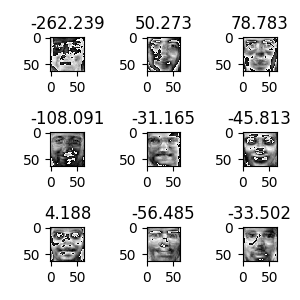
\includegraphics[height=7cm]{img/sum_of_eigenfaces.png}
	\caption{Expressing $\bX_1$ as the linear combination of the first 9 eigenfaces using \texttt{train} method of the \href{https://github.com/0xLeo/EZfaces}{EZfaces} code.}
\end{figure}
This demonstrates how eigenfaces can be visualised. Full code of the main class of the EZfaces can be found in \ref{app:ezfaces}.

%=-=-=-=-=-=-=-=-=-=-=-=-=-=-=-=-=-=-=-=-=-=-=-=-=-=-=-=-=-=-=-=-=-=-=-=-=-=-=-=-
% References
%=-=-=-=-=-=-=-=-=-=-=-=-=-=-=-=-=-=-=-=-=-=-=-=-=-=-=-=-=-=-=-=-=-=-=-=-=-=-=-=-
\newpage
\printbibliography



%=-=-=-=-=-=-=-=-=-=-=-=-=-=-=-=-=-=-=-=-=-=-=-=-=-=-=-=-=-=-=-=-=-=-=-=-=-=-=-=-
% Appendices
%=-=-=-=-=-=-=-=-=-=-=-=-=-=-=-=-=-=-=-=-=-=-=-=-=-=-=-=-=-=-=-=-=-=-=-=-=-=-=-=-
\newpage
\appendix

\section{Appendices}

% ------------------------ New appendix ------------------------ %
\newpage
\subsection{Appendix Example}
\label{app:my_pca_matlab}

\lstinputlisting[language=matlab,caption={PCA simple implementation in Matlab/ Octave. (\detokenize{src/my_pca.m)}.}]{src/my_pca.m}


% ------------------------ New appendix ------------------------ %
\newpage
\subsection{Application 1 (wine analysis) source code.}
\label{app:wine_src_code}

\lstinputlisting[language=python,caption={PCA wrapper source code. (\detokenize{src/wines/my_pca.py)}.}]{src/wines/my_pca.py}

\lstinputlisting[language=python,caption={PCA runner source code. (\detokenize{src/wines/run_my_pca.py)}.}]{src/wines/run_my_pca.py}


% ------------------------ New appendix ------------------------ %
\newpage
\subsection{Application 2 (face recognition) source code.}
\label{app:ezfaces}

\lstinputlisting[language=python,caption={Eigenfaces implementation code (\detokenize{src/face_classifier.py)}.}]{src/face_classifier.py}

\end{document}
